%%%%%%%%%%%%%%%%%%%%%%%%%%%%%%%%%%%%%%%%%%%%%%%%%%%%
% SRC
%%%%%%%%%%%%%%%%%%%%%%%%%%%%%%%%%%%%%%%%%%%%%%%%%%%%
\chapter{Short Range Correlations in Nuclei}
 As discussed in the previous chapter, the independent particle shell model (IPSM) has its great success in the description of the nuclear structure as nucleons occupying discrete energy states with their energies and momenta limited to the Fermi energy and the Fermi momentum, i.e. $\epsilon < \epsilon_{F}$ and $k<k_{F}$. However, this theory arises from a picture of a nucleons interacting only with the mean field potential generated by surrounding nucleons and it does not take into account the two-body (NN) interactions. Thus, IPSM is incapable of describing the short range properties of the NN interactions and fails to describe the structure of nuclear matter beyond the saturation density. Furthermore, measurements of the spectroscopic factors for the nuclear valence orbits via the proton knock-out experiments revealed that 30-40\% of the nuclear strength was missing compared to the predictions made by the mean field theory.
 
 Short range correlations (SRC) provide a successful explanation for the missing strength in the IPSM by considering the short distance behaviour of the NN interactions beyond the mean field, and reveal the importance of the high momentum components in the nucleon momentum distribution at $k>k_{F}$. At short distance ($\mathrm{\leq 1.0}$ fm), the attractive potential and repulsive force between nucleons excite the nucleons from their single shells and generate significant strength in the nuclear spectral functions at high momenta and energies. 
 
 To experimentally study the features of the SRC, one can use high-energy probes to directly measure the high-momentum nucleons and examine their correlations inside the nuclei. Early experiments at SLAC produced the first evidence of the SRC~\cite{SLAC_Measurement_PRC.48.2451} in inclusive electron-nucleus scattering. Recent experiments at JLab extended the study to map out the strength of the SRC in a wider range of nuclei and further examined the isospin dependence of the SRC~\cite{PhysRevLett.96.082501,PhysRevLett.99.072501,Subedi:2008zz,PhysRevLett.108.092502}. The new experiment in Hall-A at JLab, E08-014, was designed to study the structure of the SRC via inclusive electron-nucleus scattering and also to examine the isospin dependence of the SRC. 
 
 In this chapter, the features of the SRC will be discussed and the experimental techniques to explore the SRC will be briefly reviewed. 

\section{The Features of SRC}
\begin{figure}[!ht]
  \begin{center}
    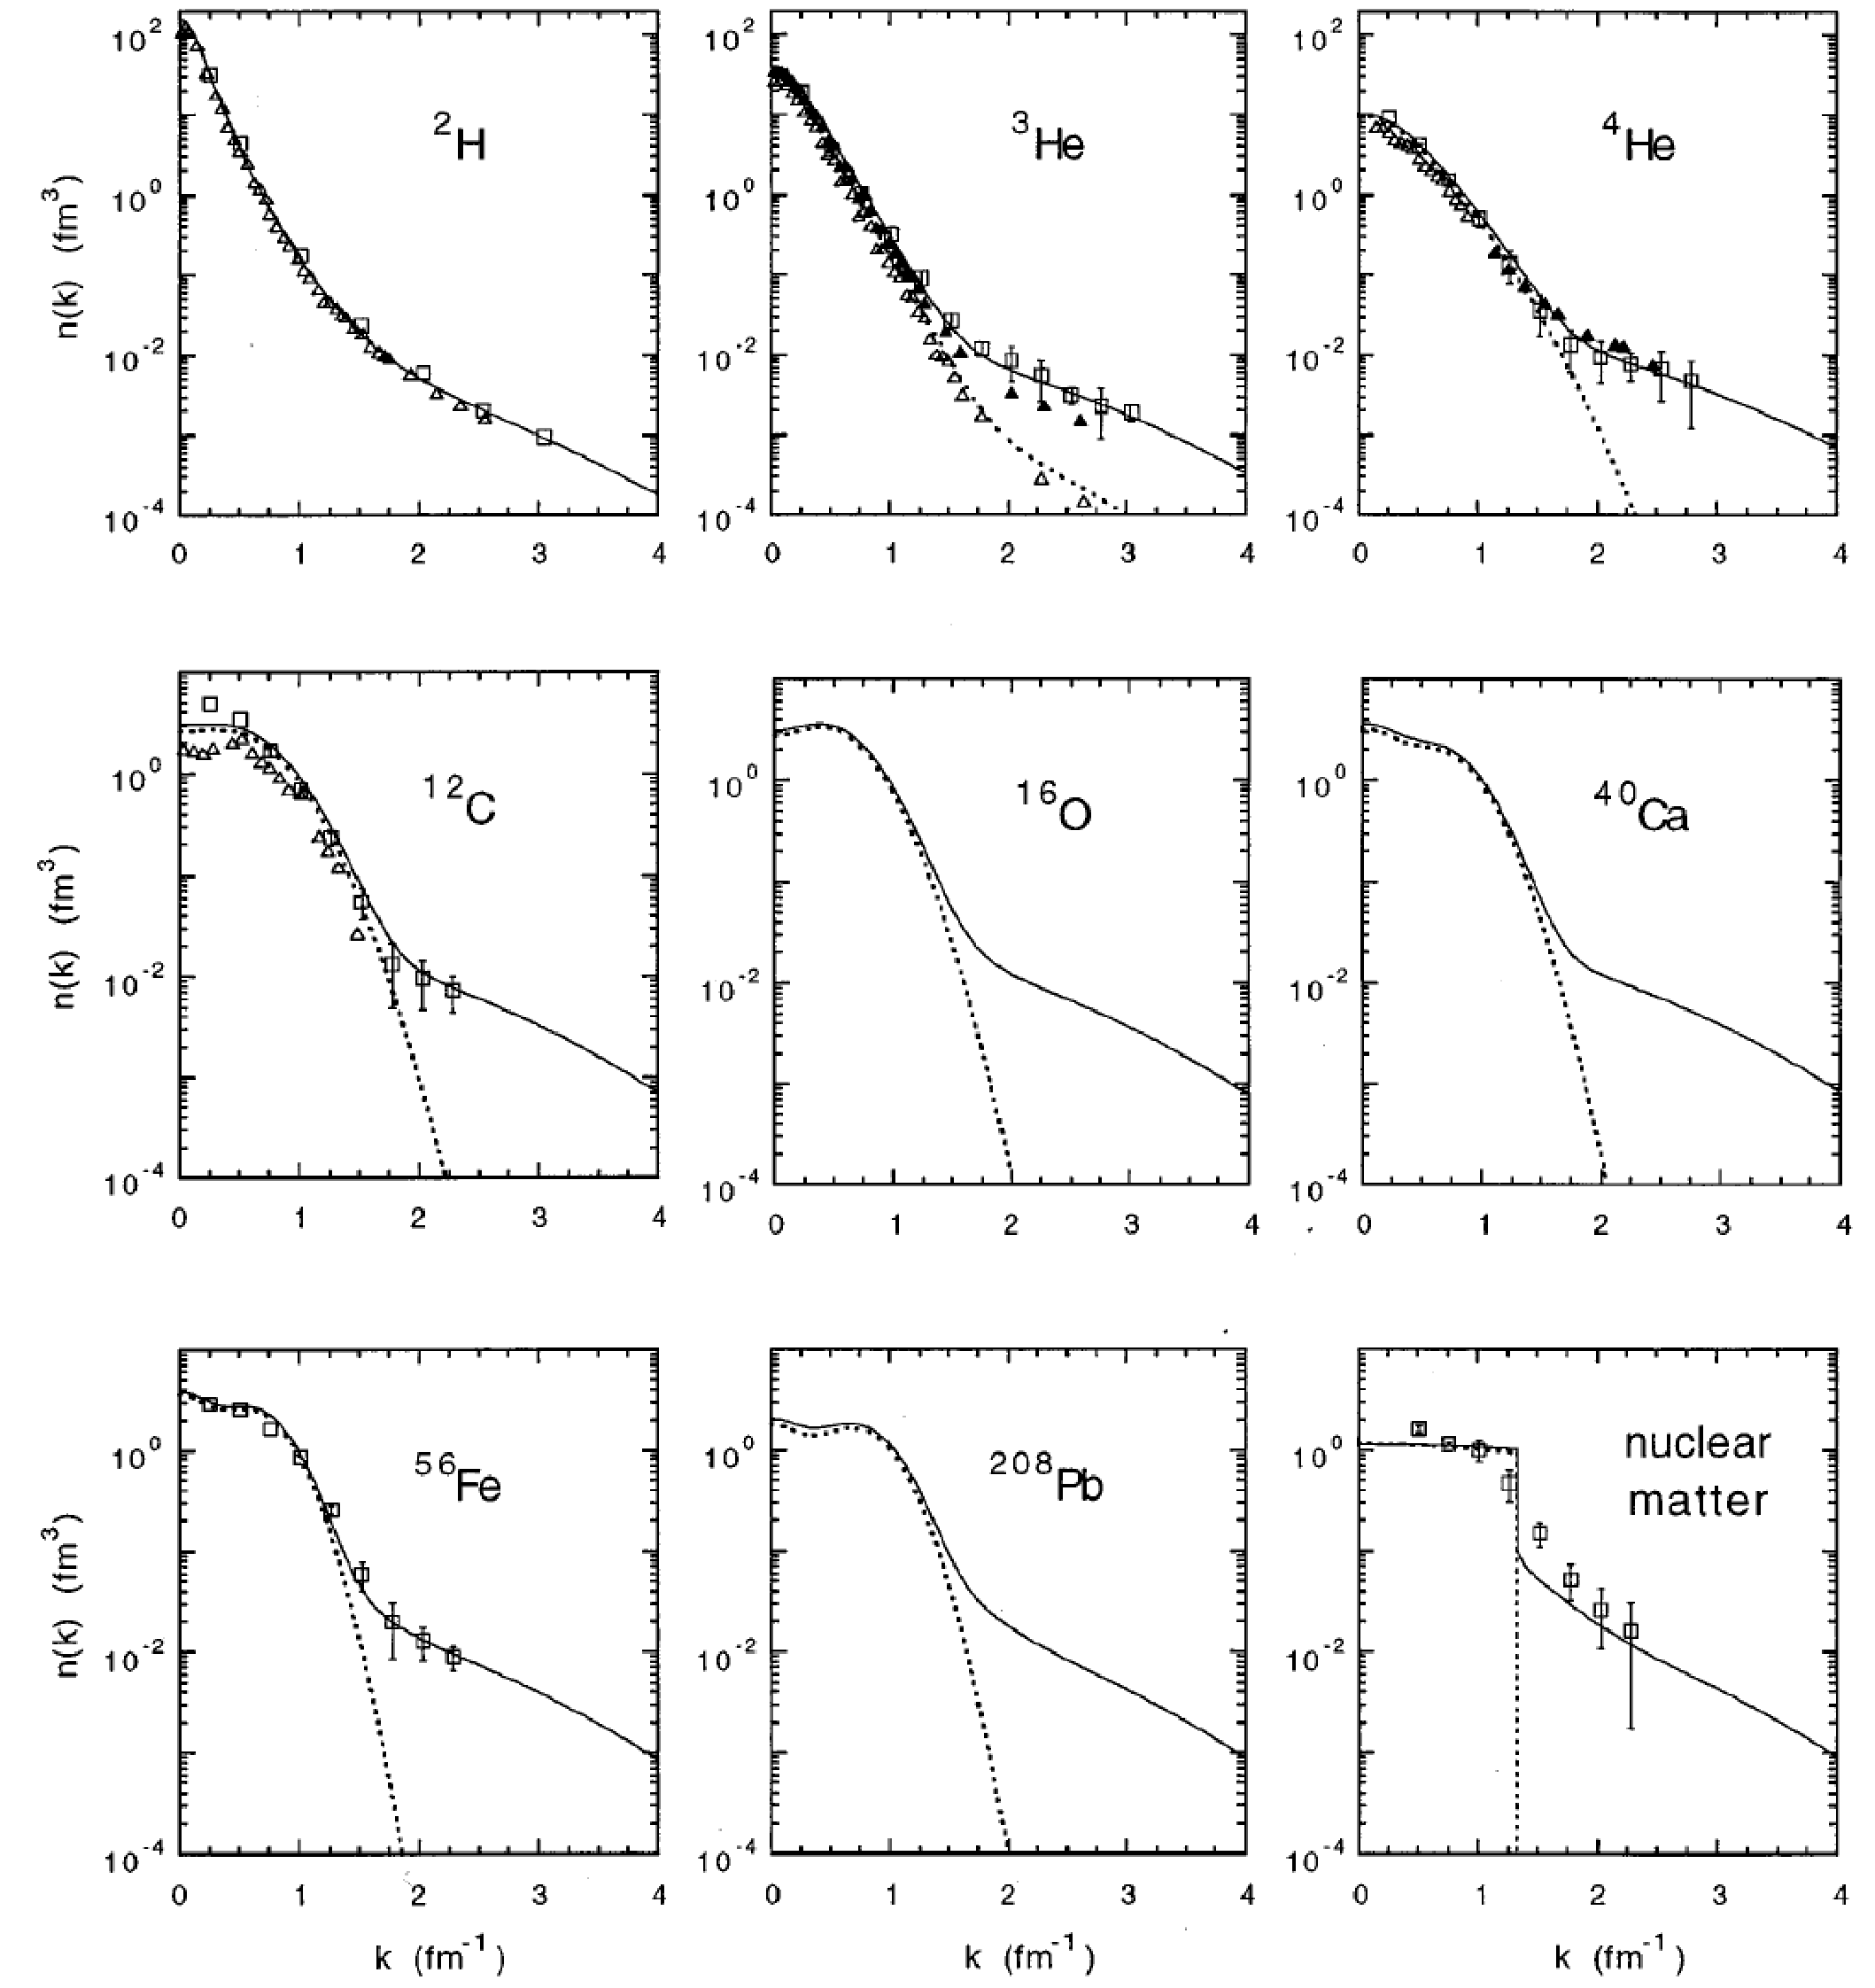
\includegraphics[type=pdf,ext=.pdf,read=.pdf,width=0.80\linewidth]{./figures/physics/Claudio_Distributions}
    \caption[Nucleon momentum distribution]{\footnotesize{Nucleon momentum distribution for various nuclei~\cite{PhysRevC.53.1689}, where dotted lines are from a mean field calculation, solid lines are the calculations including the SRC. Symbols are from experimental data. The unit of the momentum is $\mathrm{fm^{-1}}$ ($\mathrm{1~fm^{-1}\simeq 197.3~MeV/c}$). Figures were taken from Ref.~\cite{PhysRevC.53.1689}.}}
    \label{mom_dis_ox}
  \end{center}
\end{figure}

To understand how the IPSM fails to predict the nuclear strength and how the SRC contributes to an understanding of the missing nuclear strength, one needs to examine the modern theoretical nucleon momentum distributions. While the prediction made by the mean field theory gives a rapid fall-off at momenta approaching $k_{F}$, experimental results from SLAC~\cite{PhysRevC.53.1689} and elsewhere show that each nucleus has a momentum tail falling off much slower at $k>k_{F}$. The tails for all nuclei are similar from deuteron to nuclear matter, as shown in Fig.~\ref{mom_dis_ox}. 

 These results strongly contrast with the mean field prediction, but can be easily understood if these high momentum tails are generated by the short-range part of the NN interactions. In Fig.~\ref{potential_well}, nucleons interact weakly at long distance where the mean field effect dominates. The attractive force at short distance is much stronger so that the nucleons can be bound together and their wave-functions largely overlap. When the nucleons become much closer, the strong repulsive hard-core dominates the NN interactions. These short distance components of the interactions generate highly correlated nucleons in the ground states with momenta significantly larger than the Fermi momentum ($k_{F}$), which is prohibited in the IPSM. However, the total momentum of these correlated nucleons is still very small and the nucleus remains in its ground state~\cite{src_john}.

\begin{figure}[!ht]
  \begin{center}
    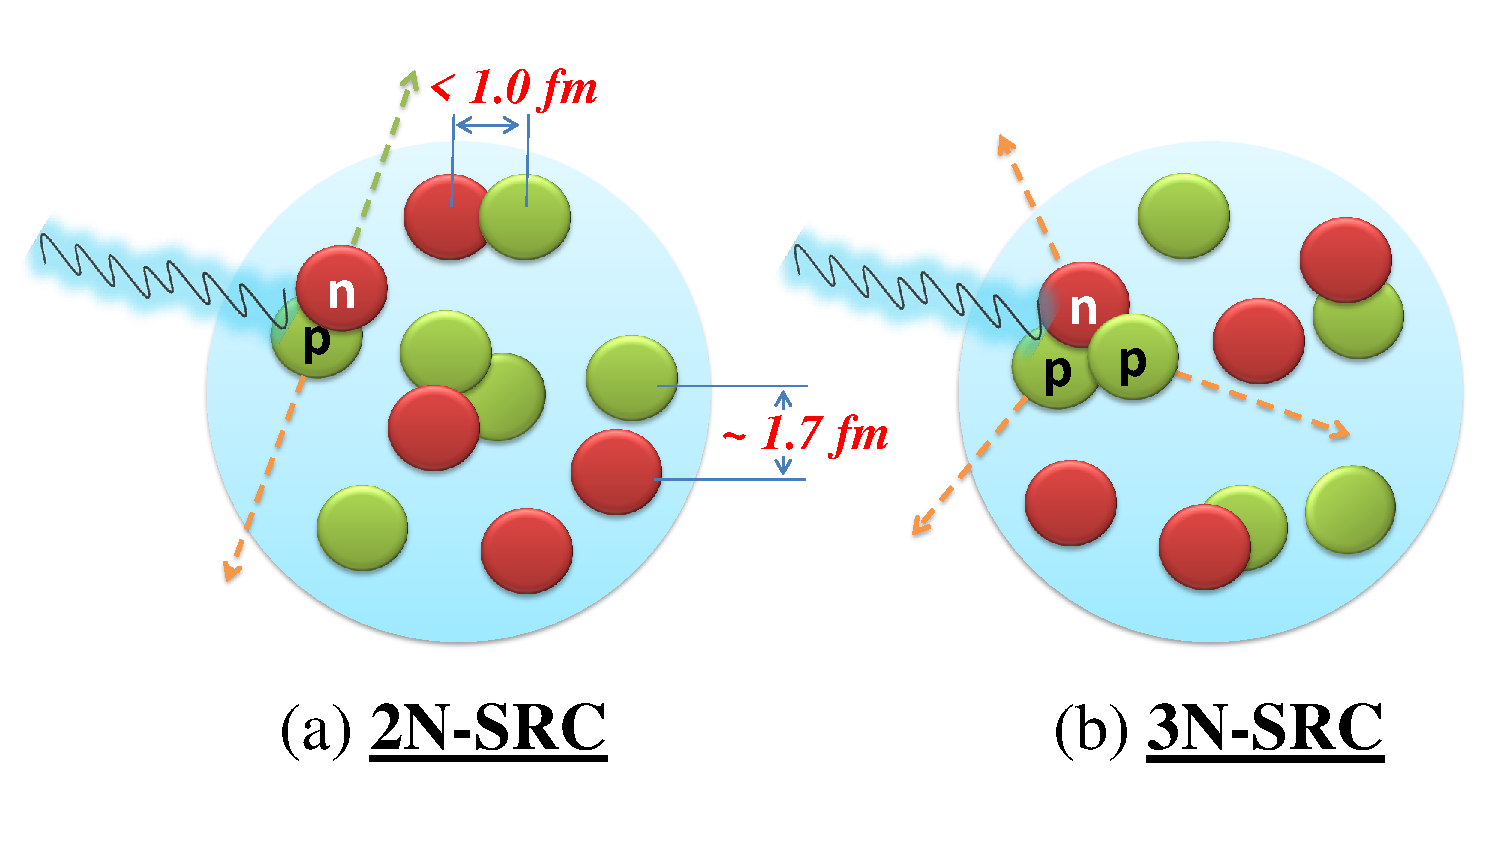
\includegraphics[type=pdf,ext=.pdf,read=.pdf,width=0.80\linewidth]{./figures/physics/2NSRC3NSRC}
    \caption[Diagrams of the 2N- and 3N-SRC]{\footnotesize{Diagram of the 2N- and 3N-SRC. On the left diagram the virtual phone breaks up the 2N-SRC pair in back-to-back ejection, and on the right diagram the break-up of  the 3N-SRC configuration results in correlated nucleon ejecting in different direction so their total momentum remains at zero.}}
    \label{2nsrc3nsrc}
  \end{center}
\end{figure}
 The asymptotic form of the momentum distribution can be broken down into several regions. At $k\leq k_{F}$, the strength is mainly contributed by the mean field potential. At large momentum, e.g. $k$ $>$ 300 MeV/c, the contribution of the mean field effect vanishes and the effect of two-nucleon short range correlation (2N-SRC) becomes dominant. These two nucleons in the configuration carry large and back-to-back momenta (Fig.~\ref{2nsrc3nsrc}.(a)), while their total center of mass momentum is modest. 

\begin{figure}[!ht]
  \begin{center}
    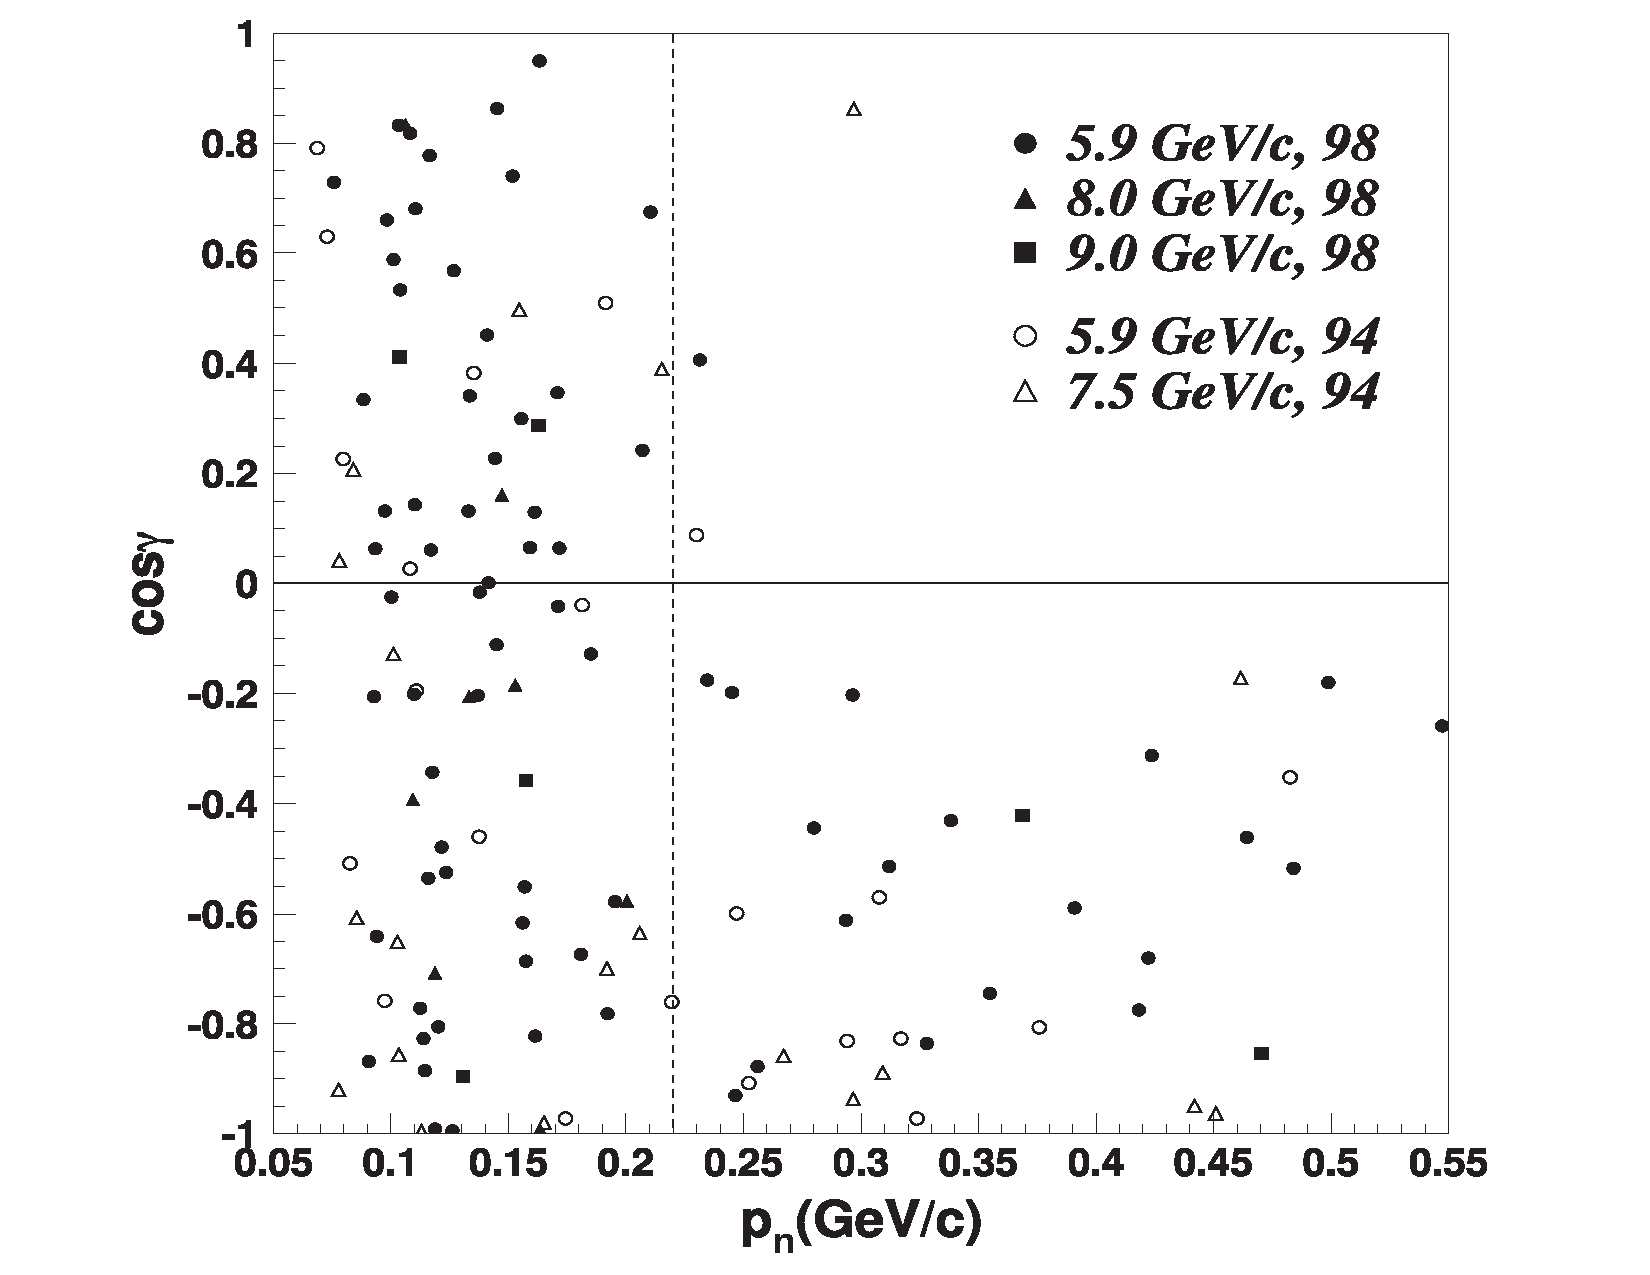
\includegraphics[type=pdf,ext=.pdf,read=.pdf,width=0.65\linewidth]{./figures/physics/2NSRC_Angle}
    \caption[Correlation between the recoil momentum and direction of neutrons in the 2N-SRC]{\footnotesize{Correlation between the recoil momentum and direction of neutrons in the 2N-SRC where $cos\gamma$ is the cosine of the opening angle between the struck nucleon and the spectator proton. Data was from the E850 at BNL with the $\mathrm{^{12}C(p,p'pn)}$ reaction. The dash line indicates the location of the Fermi momentum($k{F}$). The recoil neutrons with $p_{n}>k_{F}$ show up in the opposite direction while recoil neutrons with momenta below the Fermi momentum have no angular correlation. Plot is adopted from Ref.~\cite{PhysRevLett.90.042301}.}}
    \label{bnl_cos}
  \end{center}
\end{figure}  
 The break-up of a 2N-SRC pair must result in the strong angular correlation between these two nucleons. Such a correlation has been first observed in the E850 at Brookhaven National Lab (BNL)~\cite{PhysRevLett.90.042301} with the $\mathrm{^{12}C(p,p'pn)}$ reaction. The recoil neutron was measured in coincidence with the knocked-out proton. The opening angle (in $cos\gamma$) between the recoil neutron's momentum ($\vec{p_{n}}$) and the knock-out proton's initial momentum ($\vec{p_{i}}$) was correlated with $p_{n}$, as shown in Fig.~\ref{bnl_cos}. The result gives a uniform distribution of $cos\gamma$ for $p_{n}$ below the Fermi momentum. For $p_{n}>k_{F}$, only neutrons with $cos\gamma<0$ were observed, indicating that $\vec{p_{n}}$ is opposite to $\vec{p_{i}}$. The E01-015 in Hall-A at JLab~\cite{PhysRevLett.99.072501} used the $\mathrm{^{12}C(e,e'pn)}$ reaction and gave similar results. As shown in Fig.~\ref{triple_src_cos}, the opening angle between the knock-out proton and the recoil nucleon clearly peaks at $\mathrm{180^{o}}$ when the small center of mass motion is ignored. In addition, this experiment also discovered that these 2N-SRC pairs are dominated by $np$ configurations~\cite{Subedi:2008zz}.
\begin{figure}[!ht]
  \begin{center}
    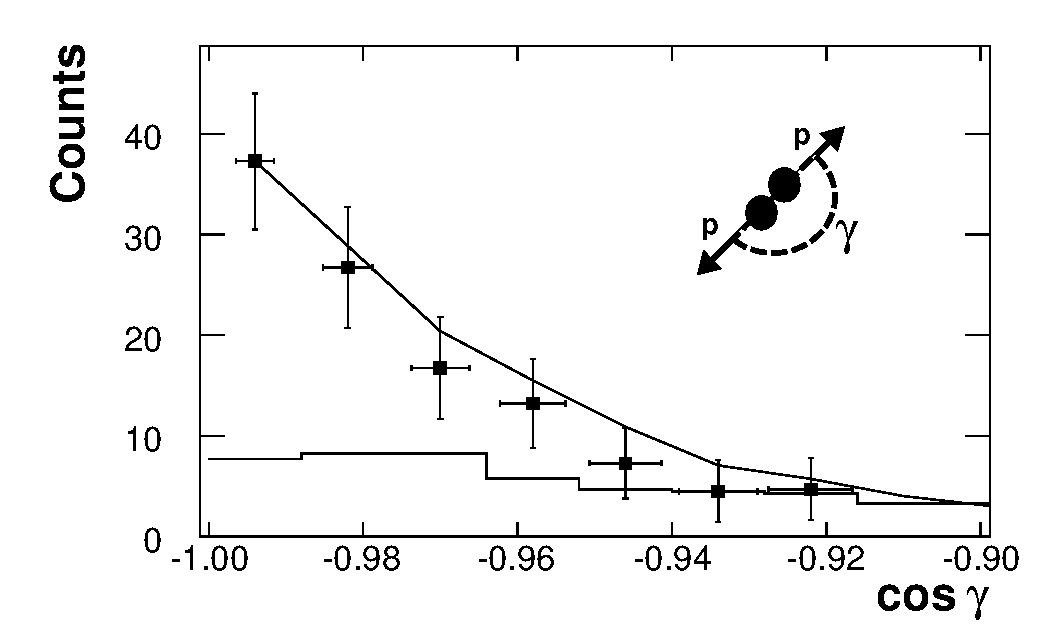
\includegraphics[type=pdf,ext=.pdf,read=.pdf,width=0.65\linewidth]{./figures/physics/10yrSRC_fig5}
    \caption[Angular correlation between nucleons in the 2N-SRC]{\footnotesize{Angular correlation between nucleons in the 2N-SRC, where the x-axis is the cosine of the opening angle between the struck nucleon with $k>k_{F}$ and the spectator nucleon in the $\mathrm{^{12}C(e,e'pp)}$ reaction. Figure is adopted from Ref.~\cite{PhysRevLett.99.072501}.}}
    \label{triple_src_cos}
  \end{center}
\end{figure}  
 
 At much higher momentum (k $\geq$ 600 MeV/c), the dominance of $np$ pairs in the SRC should be broken down since the isospin-independent repulsive core begins to prevail, and the inclusion of three-nucleon short range correlations (3N-SRC) (Fig.~\ref{2nsrc3nsrc}.(b)) may become important~\cite{src_john}. Compared with the 2N-SRC, the 3N-SRC is more difficult to observe and its configuration is much more complicated. The observation of possible 3N-SRC configurations was one of the major goals for the E08-014 and will be discussed in more details in the next section.
 
  In the limit of extremely high $k$ where the nucleon kinetic energy is comparable with the excitation energy of nucleons, non-nucleonic degree-of-freedom may need to be considered.

%%%%%%%%%%%%%%%%%%%%%%%%%%%%%%%%%%%%%%%%%%%%%%%%%%%%
% Probing SRC 
%%%%%%%%%%%%%%%%%%%%%%%%%%%%%%%%%%%%%%%%%%%%%%%%%%%%
\section{Probing SRC with Electron Scattering}
  The existence of high energy electron accelerators, e.g. NIKHEF, SLAC and JLab, provide a good opportunity to directly probe the NN short distance interactions. 
  
  The most complete experimental technique to study the 2N-SRC is the triple-coincidence measurement which not only detects the scattered electron but also maps out the momentum and angular correlations of the struck nucleon and the spectator nucleon. Due to the low counting rate, such a measurement requires a high luminosity electron beam and large acceptance spectrometers. Two experiments at JLab ~\cite{PhysRevLett.99.072501,Subedi:2008zz,E07006_pr} have successfully performed these types of measurements (Fig.~\ref{triple_src_cos}).

\begin{figure}[!ht]
  \begin{center}
    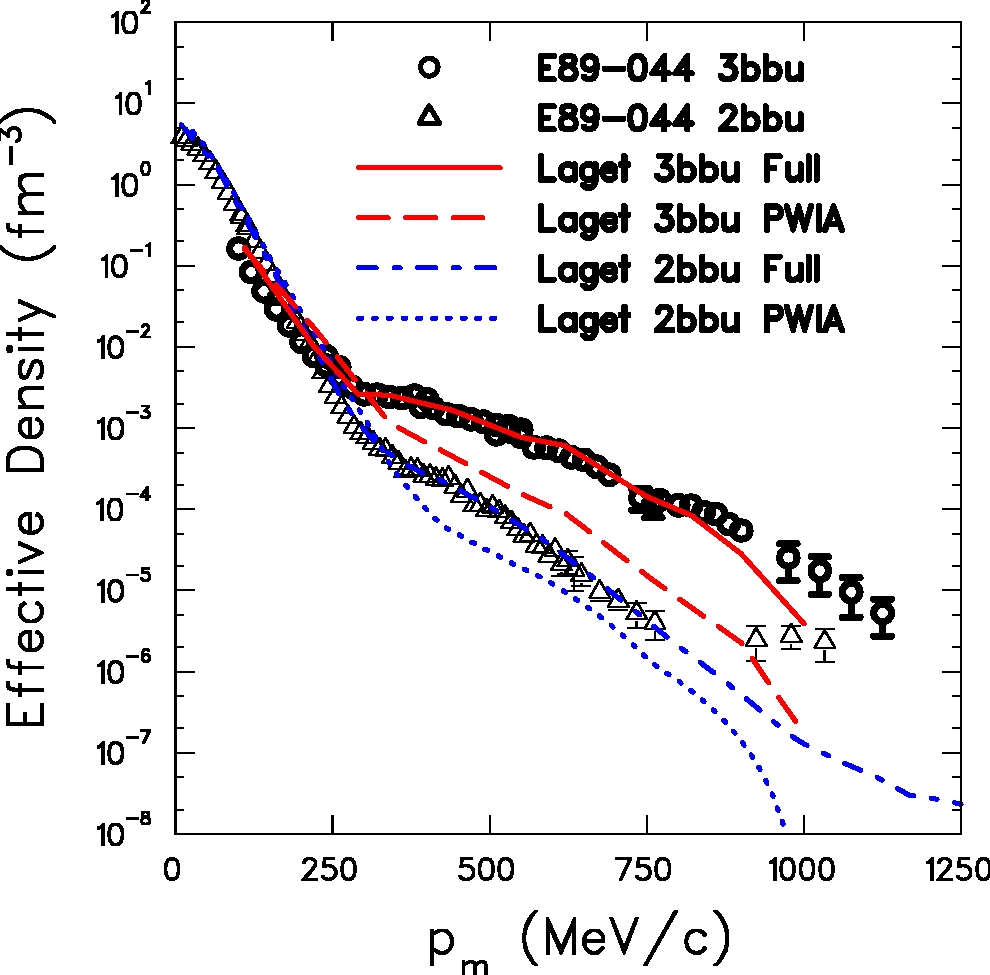
\includegraphics[type=pdf,ext=.pdf,read=.pdf,width=0.60\linewidth]{./figures/physics/10yrSRC_fig3}
    \caption[Proton effective momentum distribution in $\mathrm{^{3}He}$.]{\footnotesize{Proton effective momentum distribution in $\mathrm{^{3}He}$~\cite{PhysRevLett.94.082305}, where circles and triangles are experimental data in $\mathrm{^{3}He(e,e'p)pn}$ three-body break-up and $\mathrm{^{3}He(e,e'p)d}$ two-body break-up, respectively. Lines are theoretical calculations from~\cite{Laget200549}. Above the Fermi momentum (250 MeV), the momentum distribution of three-body break-up is much larger than the one of two-body break-up, and was explained as the combined contribution of FSI, MEC and SRC. Figure is adopted from Ref.~\cite{PhysRevLett.94.082305}}}
    \label{10yrSRC_fig3}
  \end{center}
\end{figure} 
\begin{figure}[!ht]
  \begin{center}
    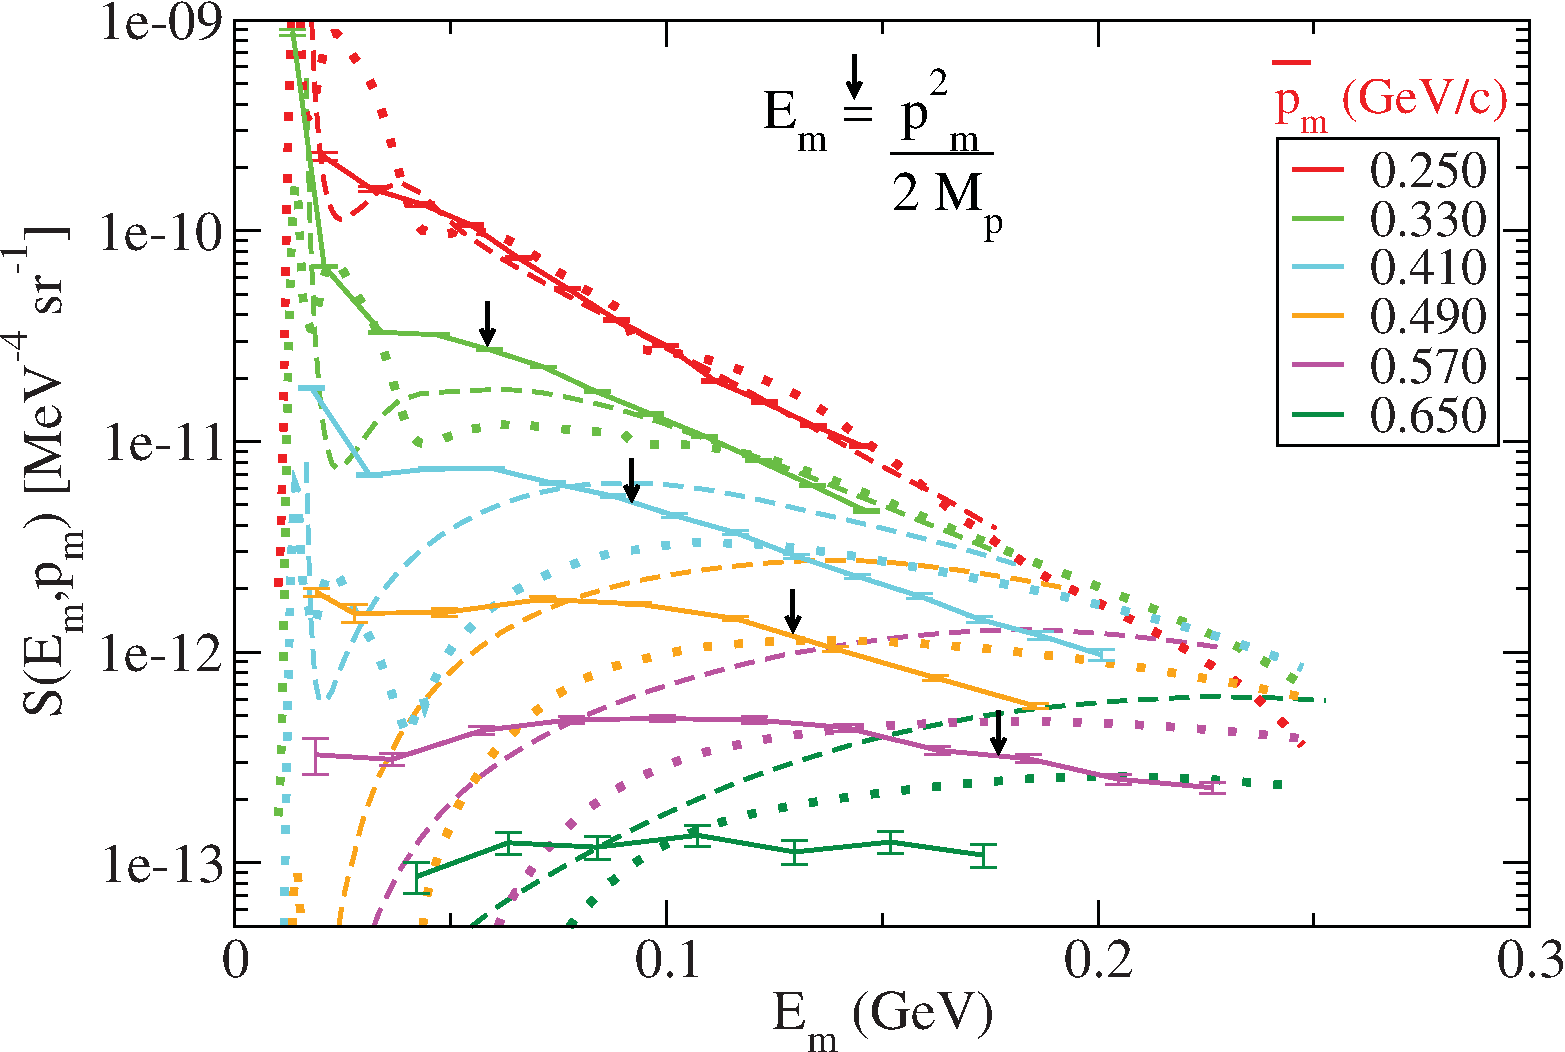
\includegraphics[type=pdf,ext=.pdf,read=.pdf,width=0.80\linewidth]{./figures/physics/Roheresults1}
    \caption[Measured distorted spectral functions for $\mathrm{^{12}C}$ from E97-006]{\footnotesize{Measured distorted spectral functions for $\mathrm{^{12}C}$ from E97-006. The data was taken in parallel kinematics to minimize the FSI. The results were compared with the theoretical predictions of the CBF~\cite{Benhar:1994hw} (dashed) and the Green's function approach~\cite{Muther:1995bk} (dotted). Figure is adopted from Ref.~\cite{PhysRevLett.93.182501}.}}
    \label{hallc_e97006}
  \end{center}
\end{figure} 
   The semi-exclusive measurement, which only detects the scattered electrons and the knocked-out protons~\cite{PhysRevLett.94.082305}, can fully probe the nuclear spectral functions (Eq.~\eqref{quasi_xs_spectral_function}) and study the dominance of the SRC and other competing processes in different kinematic regions, e.g. final-state interactions (FSI) and meson-exchange currents (MEC). NIKHEF studied the spectral function in $\mathrm{^{4}He(e,e'p)}$ data at $\mathrm{Q^{2}=0.34~GeV^{2}}$ but observed that the cross section was dominated by the long range NN interactions~\cite{vanLeeuwe1998593,Leeuwe20016}. The E89-044 in Hall-A at JLab~\cite{PhysRevLett.94.082305} measured the semi-exclusive cross sections of $\mathrm{{^{3}He}}$ at $\mathrm{Q^{2}=1.5~GeV^{2}}$. The experiment result in Fig.~\ref{10yrSRC_fig3} displays a great increase of strength in the high momentum tail which was explained as an interference between the SRC and the FSI~\cite{src_john}. The Hall-C experiment, E97-006~\cite{PhysRevLett.93.182501}, was designed to measure the spectral function at high initial energy and momentum through A(e,e'p). Special efforts were made to minimize the role of FSI by working in parallel kinematics. A sample of the results, as shown in Fig.~\ref{hallc_e97006}, agrees well with theoretical predictions.

   An inclusive measurement, where only the scattered electrons are measured, provides a powerful tool to study the feature of the SRC and probe the momentum distribution of the struck nucleon. Besides, the 3N-SRC can only be measured by the inclusive method in the current stage because of their much lower production rate and the complexity of the configurations.

\subsection{Kinematics}
  One of the key requirements to perform these experimental studies is to carefully determine the kinematic conditions and reactions, which can provide a clean measurement of high momentum nucleons and meanwhile suppress other processes such as FSI and MEC. It is also crucial to distinguish the processes of scattering off the high-momentum nucleons originally in the 2N- or 3N-SRC by varying the kinematic conditions.
    
 Although there are different kinds of reactions for probing the SRC as discussed above, these reactions share the common kinematic conditions to provide a clean study. Overall, the desire to instantly remove the nucleon from the SRC can be achieved by requiring sufficiently large energy and momentum transfer scales which significantly exceed the excitation scale of the nucleus~\cite{Frankfurt1981215,Frankfurt_misak}
\begin{equation}
  \nu >> V_{NN}, \qquad |\mathbf{q}| >> m_{N}/c,
  \label{src_condition1}
\end{equation}
where $V_{NN}$ is the characteristic potential of the NN interactions and $m_{N}$ is the nucleon mass. A reaction removing a nucleon from the nucleus under this condition allows the residual system to remain intact at the time when the nucleon in the SRC is removed, so that the properties of the SRC can be directly studied in this process.

The contribution of long range interactions, such as MEC, is suppressed by a factor of $Q^{-4}$ with respect to the production of the SRC, so they can be generally removed by requiring~\cite{M_Sargsian_JPG_29_2003}:
\begin{equation}
  Q^{2} > 1.0~GeV^{2} >> m_{meson}^{2}.
  \label{src_condition2}
\end{equation}
In this condition, intermediate state resonances still have sizeable contributions. For example, for $\mathrm{1~GeV^{2}<Q^{2}<4~GeV^{2}}$, $\gamma N\rightarrow \Delta$ transition is comparable with $\gamma N\rightarrow N$. Those resonance states are generally restricted to the region of $0<x_{bj}<1$, and their contributions can be suppressed by working at the region above the quasi-elastic (QE) peak:
\begin{equation}
  x_{bj} > 1.
  \label{src_condition3}
\end{equation}

 The combination of kinematic conditions (Eq.~\eqref{src_condition2} and Eq.~\eqref{src_condition3}) is demonstrated in Fig.~\ref{kin_cond_q2_xbj}. The plot is based on the energy and momentum conservation of the struct nucleon with different initial momenta, and the different lines represent different $\mathrm{Q^{2}}$. For scattering off nucleons in the nucleus at low $\mathrm{Q^{2}}$ (e.g. $\mathrm{0.5~GeV^{2}}$), it requires one to measure the struck nucleons at very high $x_{bj}$ (e.g. 1.8) to reach the minimum momentum requirement ($k>k_{F}$) and suppress the mean field contribution. When the $\mathrm{Q^{2}}$ is sufficiently high (e.g. $\mathrm{10~GeV^{2}}$), one can detect the struck nucleons with $k>k_{F}$ at relatively low $x_{bj}$ (e.g. 1.3). Those kinematic conditions enable a clean measurement of high momentum nucleons from the SRC.
\begin{figure}[!ht]
  \begin{center}
    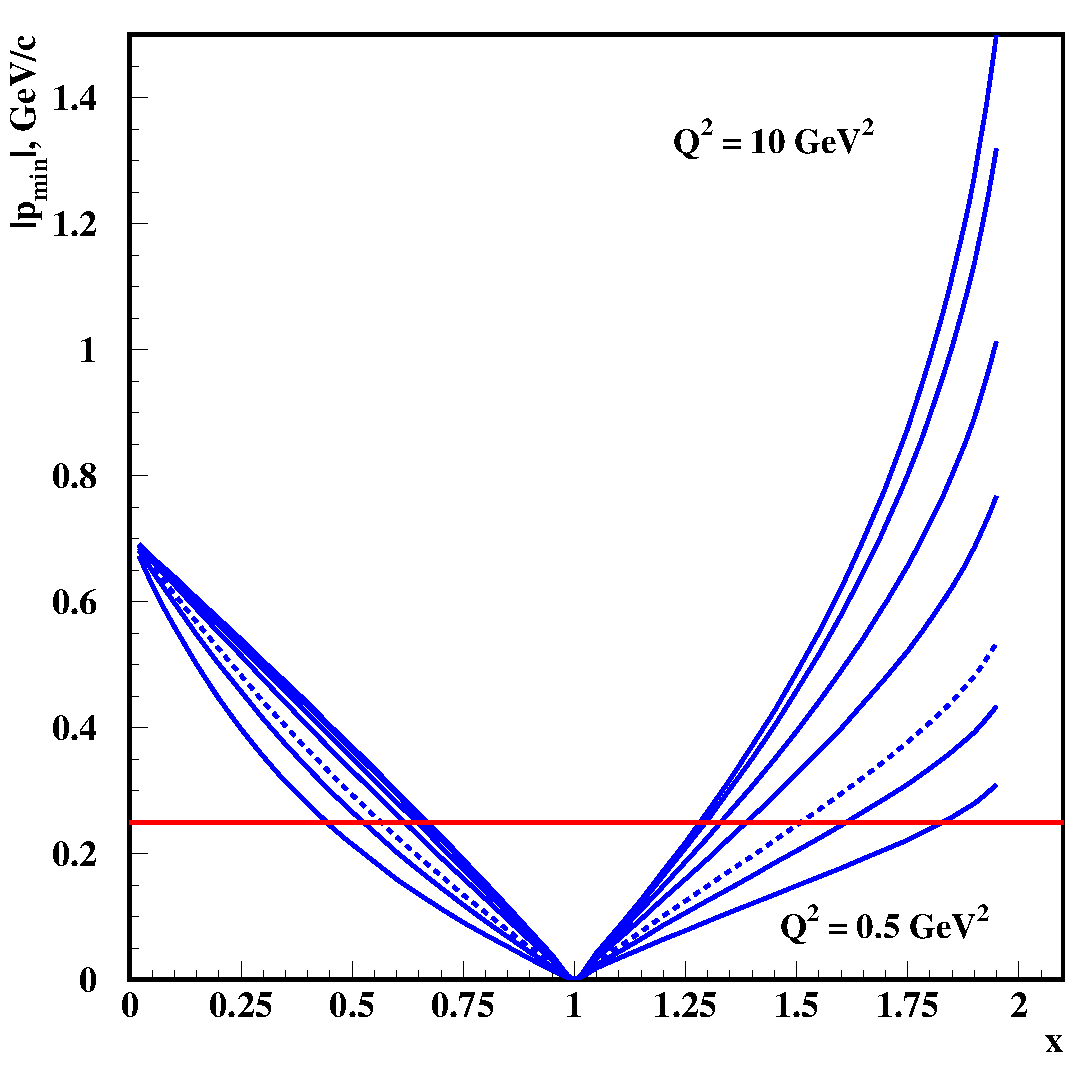
\includegraphics[type=pdf,ext=.pdf,read=.pdf,width=0.60\linewidth]{./figures/physics/kin_cond_q2_xbj}
    \caption[Minimum momentum of the struck nucleon as function of $x_{bj}$ and $\mathrm{Q^{2}}$]{\footnotesize{Minimum momentum of the struck nucleon as function of $x_{bj}$ and $\mathrm{Q^{2}}$ for scattering off a nucleon from the nucleus, where the values of $\mathrm{Q^{2}}$ from bottom to top are 0.5, 1.5, 3.0 and 10 $GeV^{2}$, respectively~\cite{Frankfurt_misak, src_john}. The red line sets the value of the Fermi momentum ($k_{F}$). Figure is adopted from Ref.~\cite{Frankfurt_misak}.}}
    \label{kin_cond_q2_xbj}
  \end{center}
\end{figure} 

%%%%%%%%%%%%%%%%%%%%%%%%%%%%%%%%%%%%%%%%%%%%%%%%%%%%%%%%%%%%%%%%%%%%%%%%%%%%%%
%%% Realistic Approach -- Start
%%%%%%%%%%%%%%%%%%%%%%%%%%%%%%%%%%%%%%%%%%%%%%%%%%%%%%%%%%%%%%%%%%%%%%%%%%%%%%
 To separate the 2N- and 3N-SRC during the scattering process, one can study the light-cone (LC) variable in the relativistic regime. A relativistic projectile moving along the z-direction probes the LC wave-function of the nucleus, $\psi_{A}(\alpha_{1},k_{1,t},...,\alpha_{i},k_{i,t},...,\alpha_{A},k_{A,t})$, where the LC variable is defined as~\cite{Frankfurt_misak}:
\begin{equation}
  \alpha_{i} = A\left(\frac{E_{i}-p_{i,z}}{E_{A}-p_{A,z}}\right)=A\left(\frac{E_{i}^{lab}-p_{i,z}^{lab}}{M_{A}}\right),
\end{equation}  
where $E_{i}$ and $p_{i,z}$ ($E_{A}$ and $p_{A,z}$) are the initial energy and longitudinal momentum of the constituent nucleon (the target nucleus $A$), respectively. $\alpha_{i}$ is invariant under Lorentz boosts in the z-direction. In the rest frame of the nucleus, $E_{A}-p_{A,z}=M_{A}$, where $M_{A}$ is the nuclear mass. 

 Similar to the definition of $x_{bj}$ in inelastic scattering (Eq.~\ref{xbj_define}), $\alpha_{i}$ denotes the LC fraction of the nucleus momentum carried by the nucleon, hence $\sum_{i}^{A}\alpha_{i}=A$. While $\alpha_{i}\leq 1$ limits the momentum fraction of the nucleon carried by the quark, to have $\alpha_{i}>1$ requires at least two nucleons involved in the scattering. Furthermore, three nucleons are required to share their momentum to have $\alpha_{i}>2$. Consequently, $\alpha_{i}$ becomes an ideal variable to distinguish the 2N-SRC from the 3N-SRC. Considering the energy and momentum conservation law for the nucleon knock-out with a virtual photon from the nucleus, one can rewrite the LC variable as~\cite{Frankfurt_misak}:
\begin{equation}
  \alpha_{i}=x_{bj}\left(1+\frac{2p_{i,z}}{\nu+|\mathbf{q}|}\right)+\frac{W_{N}^{2}-m_{i}^{2}}{2m_{i}\nu},
  \label{alpha_xbj}
\end{equation}
where $\nu$ and $\mathbf{q}$ is the energy and momentum transfer of the virtual photon, respectively, and $W_{N}^{2}=(\mathbf{p_{i}}+\mathbf{q})^{2}$. For the QE process, $W_{N}\simeq m_{i}$ yields a simple connection between $\alpha_{i}$ and $x_{bj}$. At sufficiently large $\mathrm{Q^{2}}$, $\alpha_{i}$ is usually replaced by $x_{bj}$: 
\begin{equation}
  \alpha_{i} (Q_{2}\rightarrow \infty)\rightarrow x_{bj}. 
\end{equation}
However, these two variables are different for $\mathrm{Q^{2}}$ values in few $\mathrm{GeV^{2}}$ range. One needs to examine the different scaling behaviours of the SRC as a function of $x_{bj}$ and $\alpha_{i}$ at the low $\mathrm{Q^{2}}$ region. 	
%%%%%%%%%%%%%%%%%%%%%%%%%%%%%%%%%%%%%%%%%%%%%%%%%%%%%%%%%%%%%%%%%%%%%%%%%%%%%%
%%% Realistic Approach -- End
%%%%%%%%%%%%%%%%%%%%%%%%%%%%%%%%%%%%%%%%%%%%%%%%%%%%%%%%%%%%%%%%%%%%%%%%%%%%%%

\subsection{Inclusive Measurements}
 The inclusive cross section measurement of $A(e,e')$ reaction in QE region was the first method used to isolate the SRC and currently is the only reaction to study the 3N-SRC. The cross section for $x>1.3$ and $\mathrm{Q^{2}>1~GeV^{2}}$ can be written as~\cite{Frankfurt1988235}:
\begin{eqnarray}
  \sigma_{A}(x_{bj},Q^{2}) &=& \sum_{j=2}^{A}\frac{A}{j} a_{j}(A) \sigma_{j}(x_{bj},Q^{2}) \nonumber \\
  &=& \frac{A}{2}a_{2}(A)\sigma_{2}(x_{bj},Q^{2})+\frac{A}{3}a_{3}(A)\sigma_{3}(x_{bj},Q^{2})+...,
  \label{xs_src_inclusive}
\end{eqnarray}
where $\sigma_{j}$ is the cross section for scattering off a $j$-nucleon correlation and $a_{j}(A)$ denotes the probability of finding the number of j-nucleon correlations in the nucleus. The first two terms represent the contributions from the 2N- and 3N-SRC. The 2N-SRC is expected to dominate at $1.3<x_{bj}<2$, and it generally vanishes at $x_{bj}>2$ where the 3N-SRC becomes more important.
 \begin{figure}[!ht]
  \begin{center}
    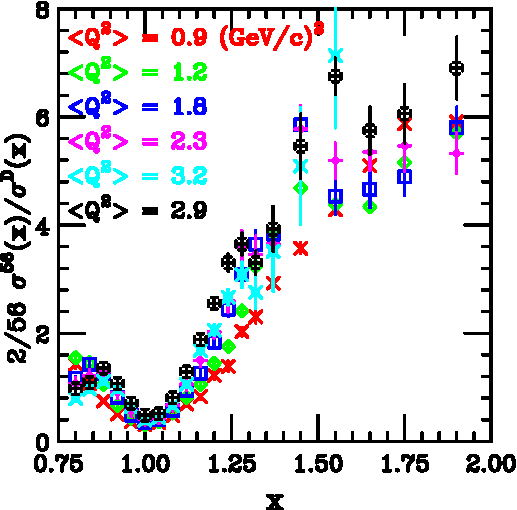
\includegraphics[type=pdf,ext=.pdf,read=.pdf,width=0.60\linewidth]{./figures/physics/SLAC_2NSRC_xbj}
    \caption[Evidence of the 2N-SRC from SLAC]{\footnotesize{Evidence of the 2N-SRC from SLAC~\cite{SLAC_Measurement_PRC.48.2451}. Each plot corresponds to the different $\mathrm{Q^{2}}$. Y-axis is the cross section ratio of $\mathrm{^{56}Fe}$ to $^{2}H$ for $\mathrm{Q^{2}=0.9-3.2~GeV^{2}}$ and x-axis is $x_{bj}$. The 2N-SRC plateau shows up at $x_{bj}>1.3$ and becomes more clear at larger $\mathrm{Q^{2}}$. Figure from Ref.~\cite{SLAC_Measurement_PRC.48.2451}.}}
    \label{SLAC_2NSRC_xbj}
  \end{center}
\end{figure}

 In the region of the 2N-SRC (3N-SRC), one expects that electron scattering off a heavy nucleus $A$ is identical to electron scattering off the deuteron-like ($\mathrm{^{3}He}$-like) configuration inside the nucleus. Hence, the inclusive cross section of the heavy nucleus $A$ is expected to scale to the one of the deuteron ($\mathrm{^{3}He}$). In the region of $1.3<x_{bj}<2.0$ where the 2N-SRC dominates, the scaling factor, $a_{2}(A)$, is given by the cross section ratio:
\begin{equation}
  a_{2}(A) = \frac{2}{A}\frac{\sigma_{A}(x_{bj},Q^{2})}{\sigma_{D}(x_{bj},Q^{2})},
  \label{src_a2}
\end{equation}
where $\sigma_{D}(x_{bj},Q^{2})$ is the inclusive cross section of electron scattering of the deuteron. Implicated in Eq.~\ref{src_a2}, $a_{2}$ in the 2N-SRC region is independent of $x_{bj}$ and $\mathrm{Q^{2}}$, and only depends on A. The value of the ratio in the scaling plateau directly gives the relative number of the 2N-SRC pairs in the nucleus compared to the deuteron.

Fig.~\ref{SLAC_2NSRC_xbj} shows the results from SLAC~\cite{SLAC_Measurement_PRC.48.2451}, which for the first time observed such a plateau with the cross section ratio of $\mathrm{^{56}Fe}$ to $\mathrm{^{2}H}$ at $x_{bj}>1.5$ and $\mathrm{Q^{2}=0.9-3.2~GeV^{2}}$. Other targets, $\mathrm{^{4}He}$, $\mathrm{^{27}Al}$ and $\mathrm{^{64}Cu}$ were also studied and all showed clear evidences of the 2N-SRC plateaus. However, Fig.~\ref{SLAC_2NSRC_xbj} also suggests a $\mathrm{Q^{2}}$ dependence of $a_{2}$. The statistics were limited and the deuteron data was taken at different kinematics, so the result was extracted with nontrivial extrapolations. Recent Jefferson Lab results from the E89-008~\cite{Arrington:2003tw, Arrington:2006pn} and the E02-019~\cite{PhysRevLett.108.092502} in Hall-C, and Large Acceptance Spectrometer (CLAS)~\cite{PhysRevLett.96.082501} in Hall-B extracted the values of $a_{2}$ from various nuclei with higher statistics and better resolution, and their results indicate a sound agreement in the 2N-SRC region (Fig.~\ref{CLAS_2NSRC_3NSRC} and Fig.~\ref{E02019_2NSRC_3NSRC}). 
\begin{figure}[!ht]
  \begin{center}
    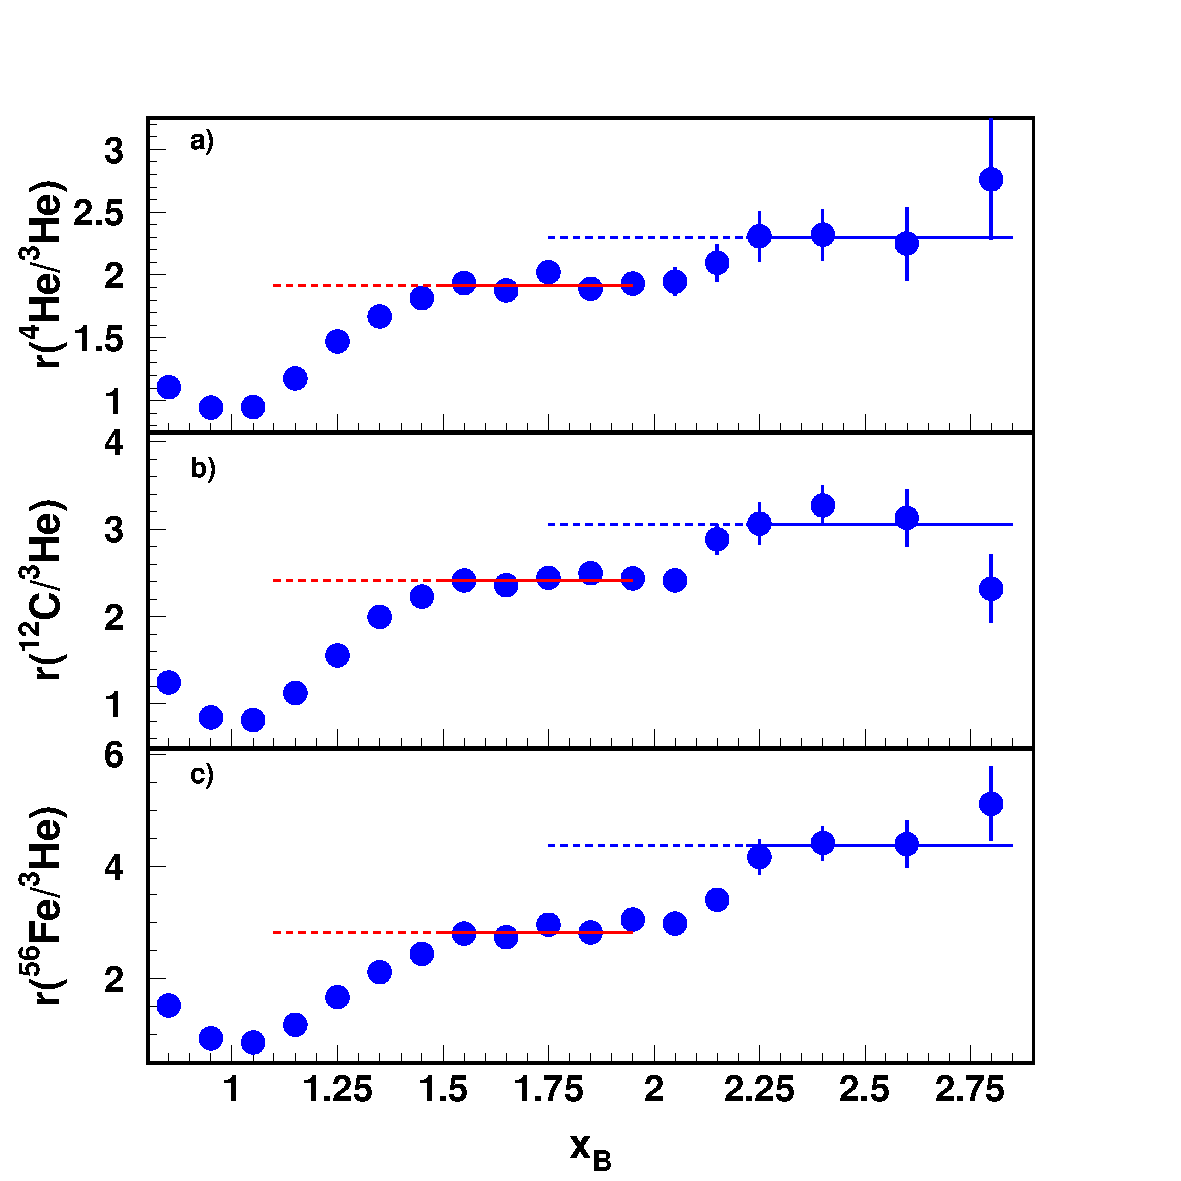
\includegraphics[type=pdf,ext=.pdf,read=.pdf,width=0.70\linewidth]{./figures/physics/CLAS_2NSRC_3NSRC}
    \caption[2N- and 3N-SRC results from CLAS in Hall-B]{\footnotesize{2N- and 3N-SRC results from CLAS Hall-B~\cite{PhysRevLett.96.082501}. The top, middle and bottom plots give the cross section ratios of $\mathrm{^{4}He}$, $\mathrm{^{12}C}$ and $\mathrm{^{56}Fe}$ to $\mathrm{^{3}He}$, respectively. In each plot, both the 2N-SRC plateau (in $1.5<x_{bj}<2$) and the 3N-SRC plateau (in $x_{bj}>2$) can be observed. Figure are reproduced from the original plots in Ref.~\cite{PhysRevLett.96.082501}.}}
    \label{CLAS_2NSRC_3NSRC}
  \end{center}
\end{figure} 

Similarly, one can study the scaling factor, $a_{3}(A)$, in the 3N-SRC at $2<x_{bj}<3$ with the cross section ratio of the heavy nucleus to $\mathrm{^{3}He}$:
\begin{equation}
  a_{3}(A) = K\cdot\frac{3}{A}\frac{\sigma_{A}(x_{bj},Q^{2})}{\sigma_{^{3}He}(x_{bj},Q^{2})},
  \label{src_a3}
\end{equation}
which denotes the number of $\mathrm{^{3}He}$-like 3N-SRC configuration in the nucleus. $K$ corrects for the difference of the electron-proton and electron-neutron cross sections:
\begin{equation}
  K = \frac{\sigma_{ep}+\sigma_{en}}{Z\sigma_{ep}+(A-Z)\sigma_{en}}.
\end{equation}

\begin{figure}[!ht]
  \begin{center}
    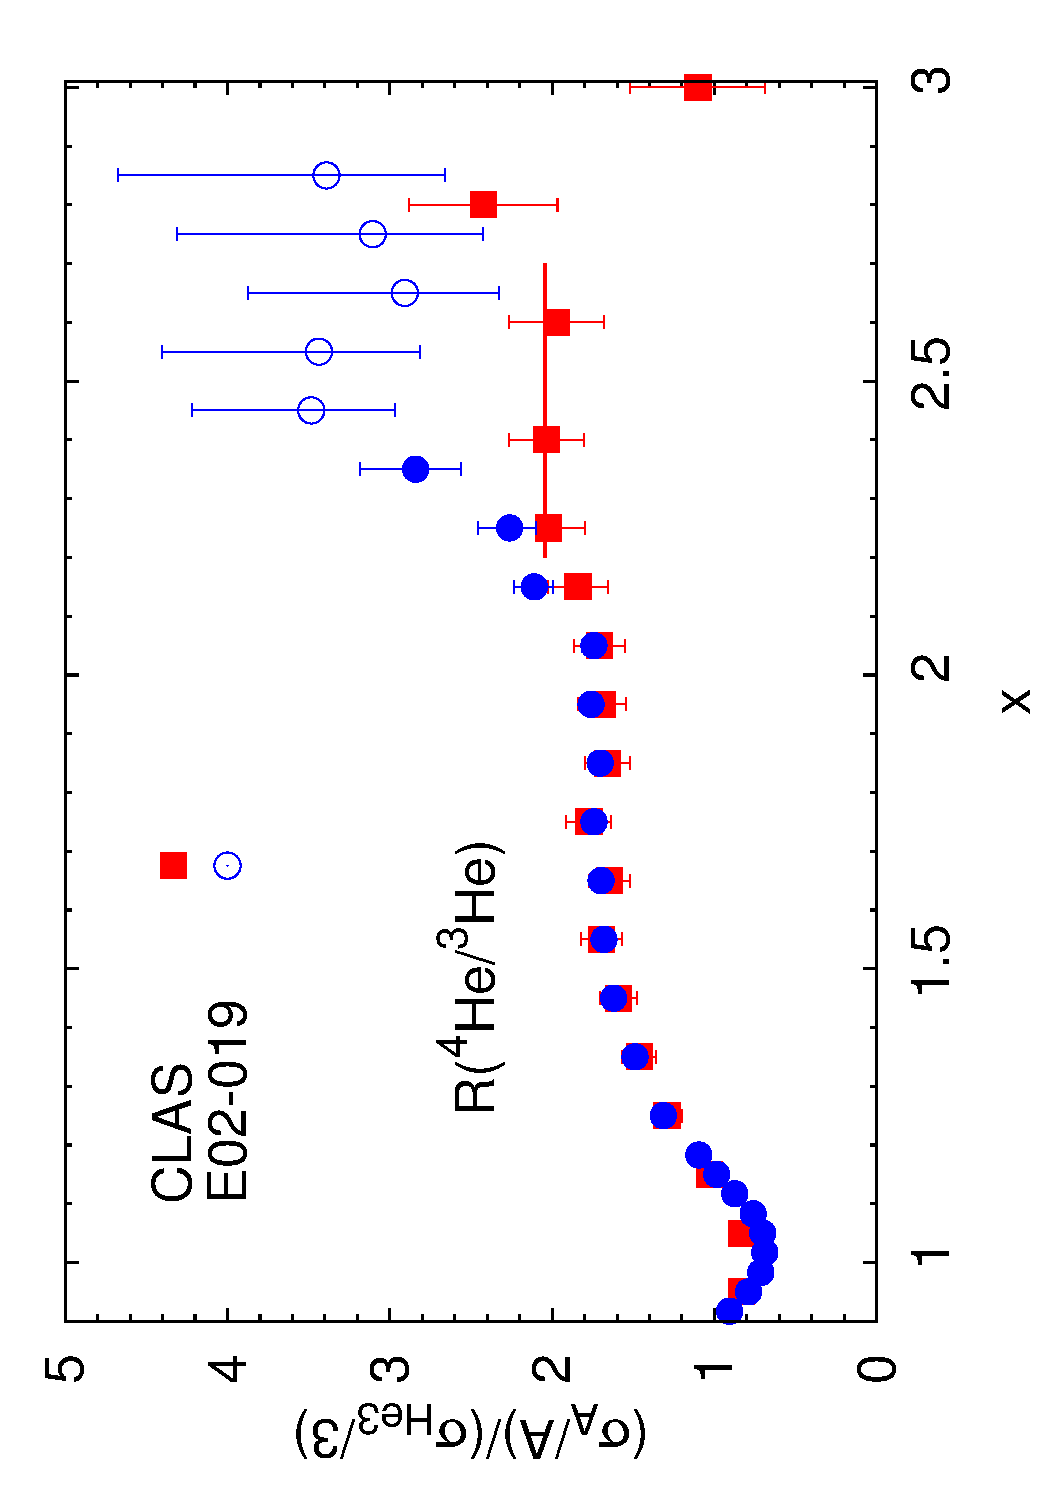
\includegraphics[type=pdf,ext=.pdf,read=.pdf,angle=270.,width=0.80\linewidth]{./figures/physics/E02019_2NSRC_3NSRC}
    \caption[2N- and 3N-SRC in $\mathrm{^{4}He/^{3}He}$ from the E02-019]{\footnotesize{2N- and 3N-SRC in $\mathrm{^{4}He/^{3}He}$ from the E02-019 in Hall-C compared with the result from Hall-B, where the blue dots are the E02-019 data and red dots are the CLAS data. Figure is adopted from Ref.~\cite{PhysRevLett.108.092502}.}}
    \label{E02019_2NSRC_3NSRC}
  \end{center}
\end{figure} 
In the CLAS data, the kinematics was for the first time extended into the region of 3N-SRC and a plateau at $x_{bj}>2.3$ was observed. The E02-019 data, however, yields a different result in this region. From Fig.~\ref{E02019_2NSRC_3NSRC}, the cross section ratio of $\mathrm{^{4}He/^{3}He}$ reaches the scaling region at $x_{bj}>2.5$, slightly later than the CLAS result, and the scaling plateau can not be clearly identified because of the large error bars. An explanation of the discrepancy is not straightforward since these two experiments ran at very different $\mathrm{Q^{2}}$ ranges ($\mathrm{Q^{2}\sim 1.6~GeV^{2}}$ for CLAS and $\mathrm{Q^{2}\sim 2.7~GeV^{2}}$ for the E02-019). It is unclear whether these measurements isolated the 3N-SRC contributions or not. The E08-014 in Hall-A focuses on studying the scaling of 3N-SRC at $x_{bj}>2$ with much better accuracy, and the new preliminary results will be presented later. 

\begin{figure}[!h]
  \begin{center}
        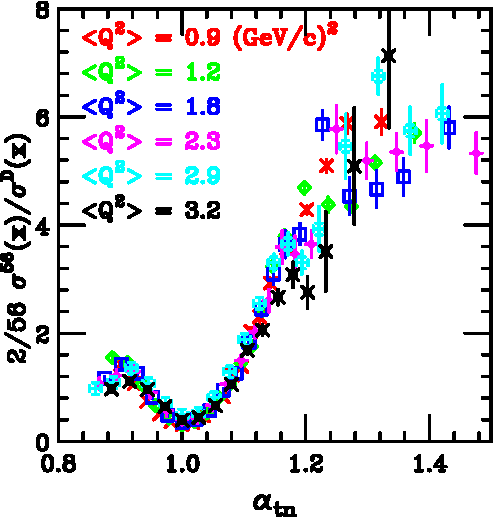
\includegraphics[type=pdf,ext=.pdf,read=.pdf,width=0.6\linewidth]{./figures/physics/SLAC_2NSRC_alpha}
        \caption[Ratio of $\mathrm{^{56}Fe/^{2}H}$ as a function of $\alpha_{2N}$ from SLAC]{\footnotesize{Ratio of $\mathrm{^{56}Fe/^{2}H}$ as a function of $\alpha_{2N}$ for different $\mathrm{Q^{2}}$ values~\cite{SLAC_Measurement_PRC.48.2451}. $\alpha_{2N}$ (labelled as $\alpha_{tn}$ in this plot) is an approximation of the LC variable by assuming the total momentum of the nucleons in the 2N-SRC is zero. Compared with Fig.~\ref{SLAC_2NSRC_xbj}, $\alpha_{2N}$ provides better scaling behaviour and indicates less $\mathrm{Q^{2}}$ dependence.}}
    \label{SLAC_2NSRC_alpha}
  \end{center}
\end{figure}
The other important element in the study of the SRC in inclusive measurements is the difference between two scaling variables, $x_{bj}$ and $\alpha_{i}$. From Eq.~\eqref{alpha_xbj}, the LC variable $\alpha_{i}$ is approximately equal to $x_{bj}$ at large $\mathrm{Q^{2}}$. At the few $\mathrm{GeV^{2}}$ level, the approximation is invalid and the difference in the scaling behaviour of the SRC ratios as a function of $x_{bj}$ and $\alpha_{i}$ must be carefully examined. 

Although $\alpha_{i}$ can not be reconstructed in inclusive scattering, one can assume that in the PWIA the virtual photon interacts with the nucleon in a 2N-SRC pair at rest. This assumption leads to a new expression of the LC variable specifically for the 2N-SRC:
\begin{equation}
  \alpha_{2N} = 2-\frac{q_{-}+2m}{2m}\frac{\sqrt{W^{2}-4m^{2}}+W}{W},  
\end{equation}
where $q_{-}$ is the initial longitudinal momentum of the struck nucleon and $W^{2}=4m_{N}^{2}+4m_{N}\nu-Q^{2}$. 

The analysis of SLAC data~\cite{SLAC_Measurement_PRC.48.2451} reveals that compared with $x_{bj}$ in Fig.~\ref{SLAC_2NSRC_xbj}, $\alpha_{2N}$ can better isolate the 2N-SRC (Fig.~\ref{SLAC_2NSRC_alpha}) and allow one to examine the transition region from the 2N-SRC to the 3N-SRC. A more general expression for all $\alpha_{i}$~\cite{e08014_pr} in the inclusive measurement can be obtained from:
\begin{equation}
  q_{-}\cdot\alpha_{jN}m_{N}+q_{+}\cdot\left(M_{A}-\frac{M_{r}^{2}}{m_{N}(j-\alpha_{jN})}\right)=m_{N}^{2},
\end{equation}
where $j=2,3,...$. $q_{+}$ is the initial transverse momentum of the struck nucleon and $M_{r}$ is the mass of the residual system. Taking $j=3$, one can solve for $\alpha_{3N}$, but the exact expression depends on the value of $M_{r}$ which is difficult to specify since the 3N-SRC is a more complicated configuration.

 In general, there are two types of 3N-SRC, as shown in Fig.~\ref{3nsrc_two_types}. In the first type, namely 3N-SRC-I, the total initial momentum of two nucleons is equal to that of the struck nucleon but in the opposite direction. This configuration is similar to the 2N-SRC but involving in three nucleons. The second type, 3N-SRC-II, refers to the configuration of three nucleons carrying momenta all exceeding the Fermi momentum in three different directions. Although the 3N-SRC-II configuration is easier to be observed experimentally via semi-exclusive reactions, it is less likely to occur than the 3N-SRC-I one since it requires a larger separation energy~\cite{Frankfurt_misak}.
 
 The situation of the 3N-SRC-I, where $M_{r}=2m_{N}$, gives:
\begin{equation}
  \alpha_{3N-I} = \frac{3}{2}+\frac{1}{2}[\sqrt{ (3+b_{1})^{2}-b_{2}}-b_{1}],
\end{equation} 
where,
\begin{equation}
  b_{1} = \frac{q_{+}}{q_{-}} \frac{M_{A}}{m_{N}}-\frac{m_{N}}{q_{-}},\qquad b_{2} = 16 \frac{q_{+}}{q_{-}}.
\end{equation} 
The value of $M_{r}$ becomes larger for the 3N-SRC-II, and its LC variable, $\alpha_{3N-II}$, has a more complicated form. Examining the scaling as a function of $\alpha_{3N-I}$ and $\alpha_{3N-II}$ by varying the value of $M_{r}$ provides a sensitive probe to the detailed structure of 3N-SRC~\cite{e08014_pr}.
\begin{figure}[h]
	  \begin{center}
	    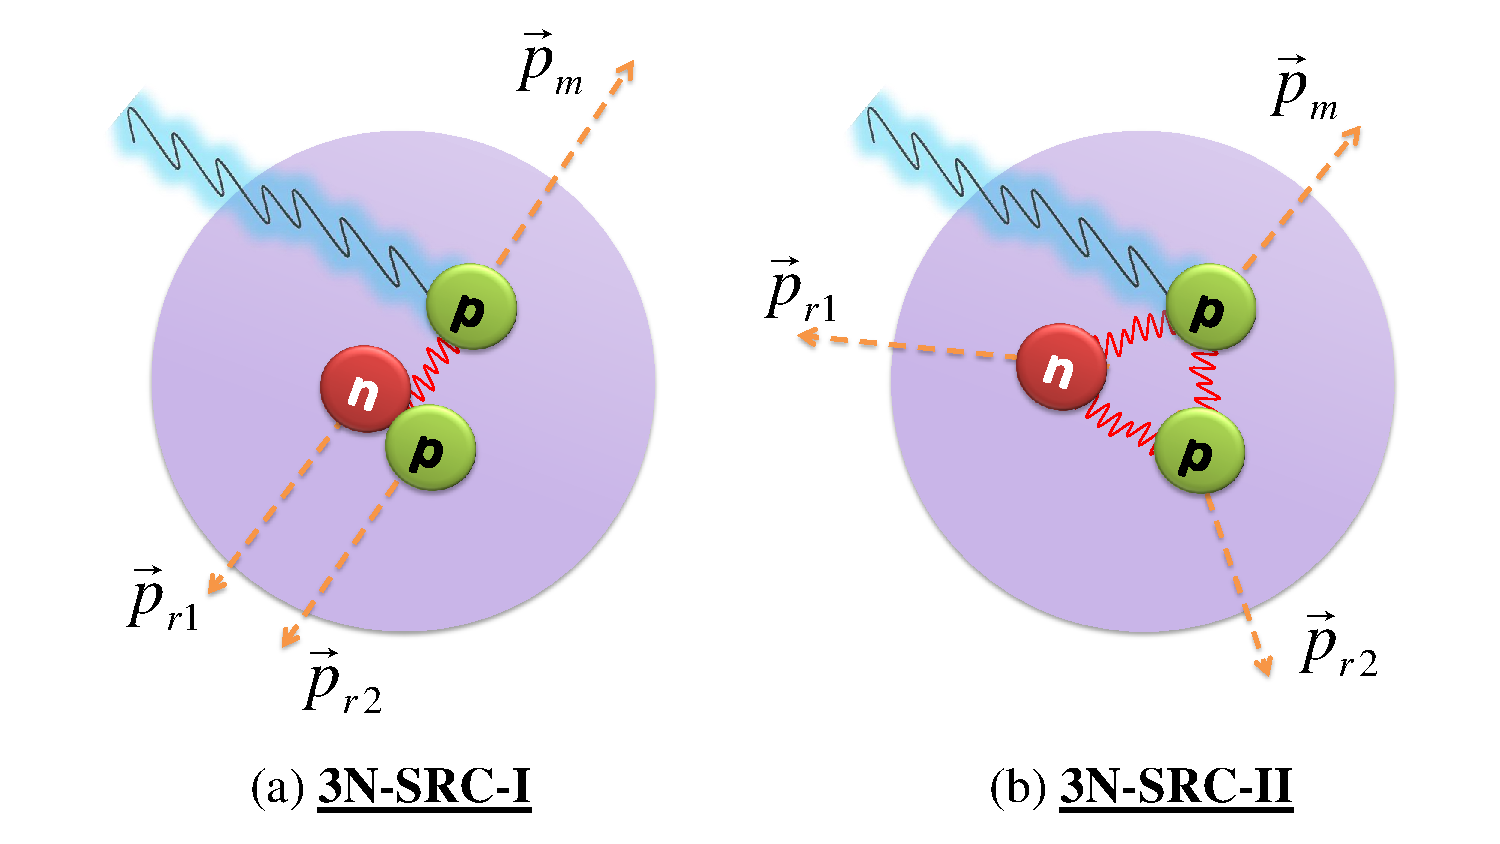
\includegraphics[type=pdf,ext=.pdf,read=.pdf,width=0.80\linewidth]{./figures/physics/3nsrc_two_types}
	    \caption[Two types of 3N-SRC configuration]{\footnotesize{Two types of 3N-SRC configuration~\cite{Frankfurt_misak}.}}
	  \label{3nsrc_two_types}
	  \end{center}
\end{figure} 
\subsection{Isospin Dependence}
\begin{figure}[!ht]
  \begin{center}
    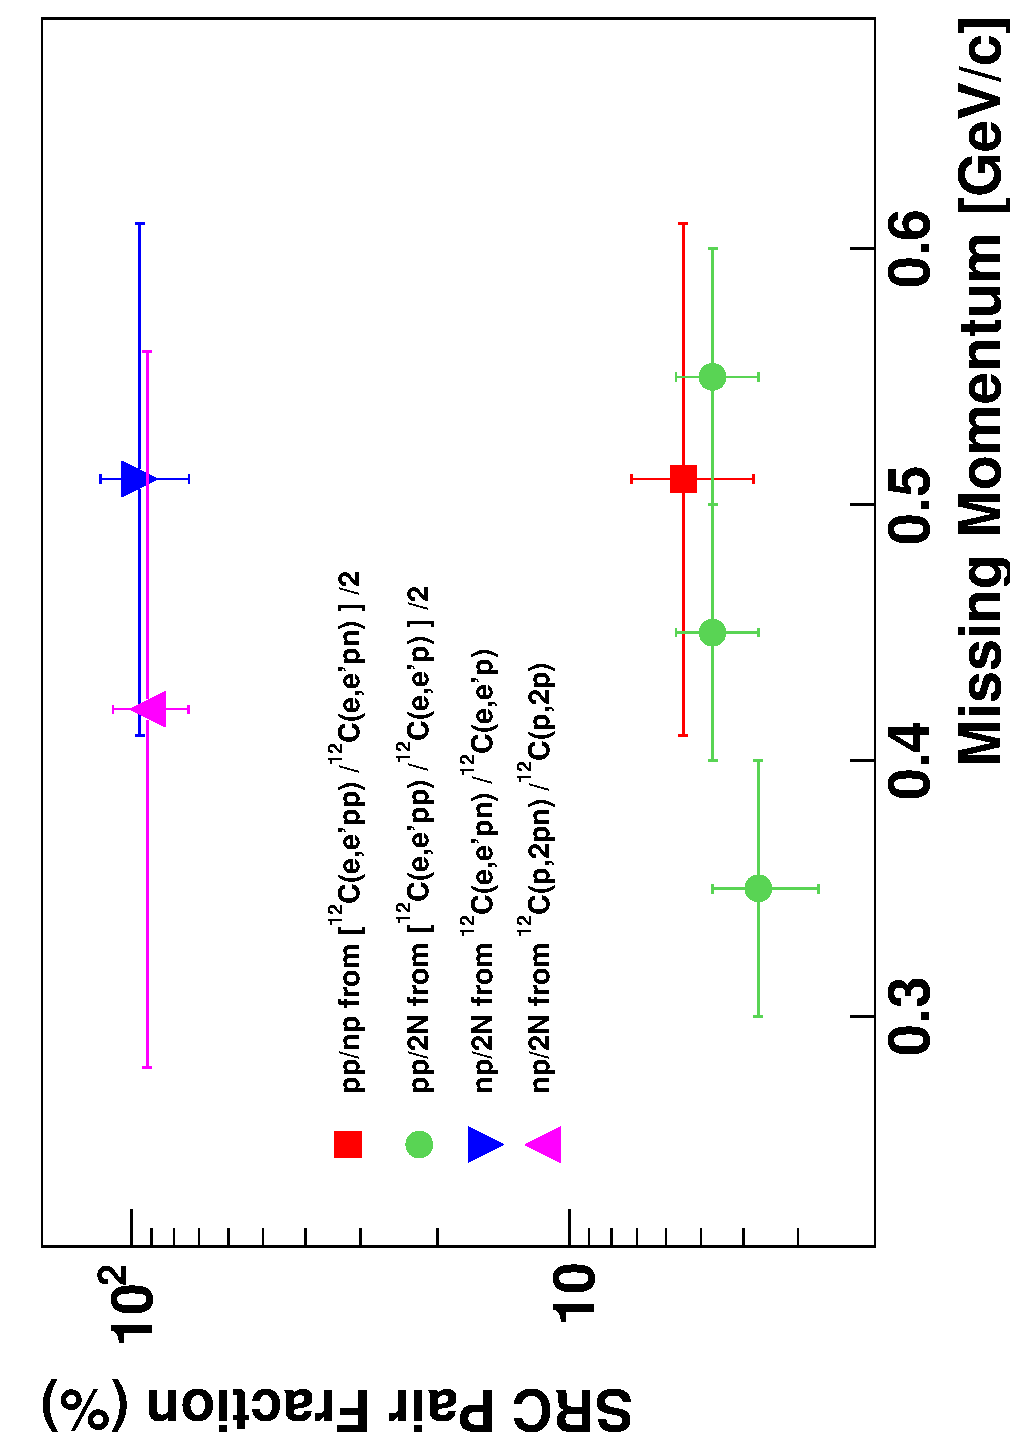
\includegraphics[type=pdf,angle=270,ext=.pdf,read=.pdf,width=0.80\linewidth]{./figures/physics/10yrSRC_fig7}
    \caption[The fraction of $np$ pairs to $pp$ pairs in the 2N-SRC]{\footnotesize{The fraction of $np$ pairs to $pp$ pairs in the 2N-SRC in carbon from the triple-coincidence experiment in Hall-A. Figure is adopted from Ref.~\cite{Subedi:2008zz}.}}
    \label{triple_src_np}
  \end{center}
\end{figure} 
  In the early analysis of inclusive measurements where the struck nucleon was not identified,  isospin-independence was assumed and the ratio of neutrons to protons in the SRC configurations was treated to be equal to the $N/Z$ ratio. 

  Triple-coincidence experiments at JLab~\cite{PhysRevLett.90.042301,PhysRevLett.99.072501,Subedi:2008zz} studied the isospin effect by measuring the ratio of $pn$ and $pp$ in the 2N-SRC with the $\mathrm{^{12}C(e,e'pp)}$ and $\mathrm{^{12}C(e,e'pn)}$ reactions. As shown in Fig.~\ref{triple_src_np}, the result~\cite{Subedi:2008zz} revealed that the ratio of $np/pp$ pairs is around $\mathrm{18\pm 5}$. The dominance of $np$ pairs indicates that the assumption of the isospin independence is invalid.  
  
  Numerical studies~\cite{PhysRevC.72.054310} suggest that because of the tensor interaction, the 2N-SRC pairs should be mainly in iso-singlet ($np$ with T=0) states. The iso-triplet ($pp$,$np$ and $nn$ with $T=1$) pairs experience a much smaller attractive component in the NN potential till they are close enough to interact via the repulsive core.
 
\begin{figure}[!ht]
  \begin{center}
    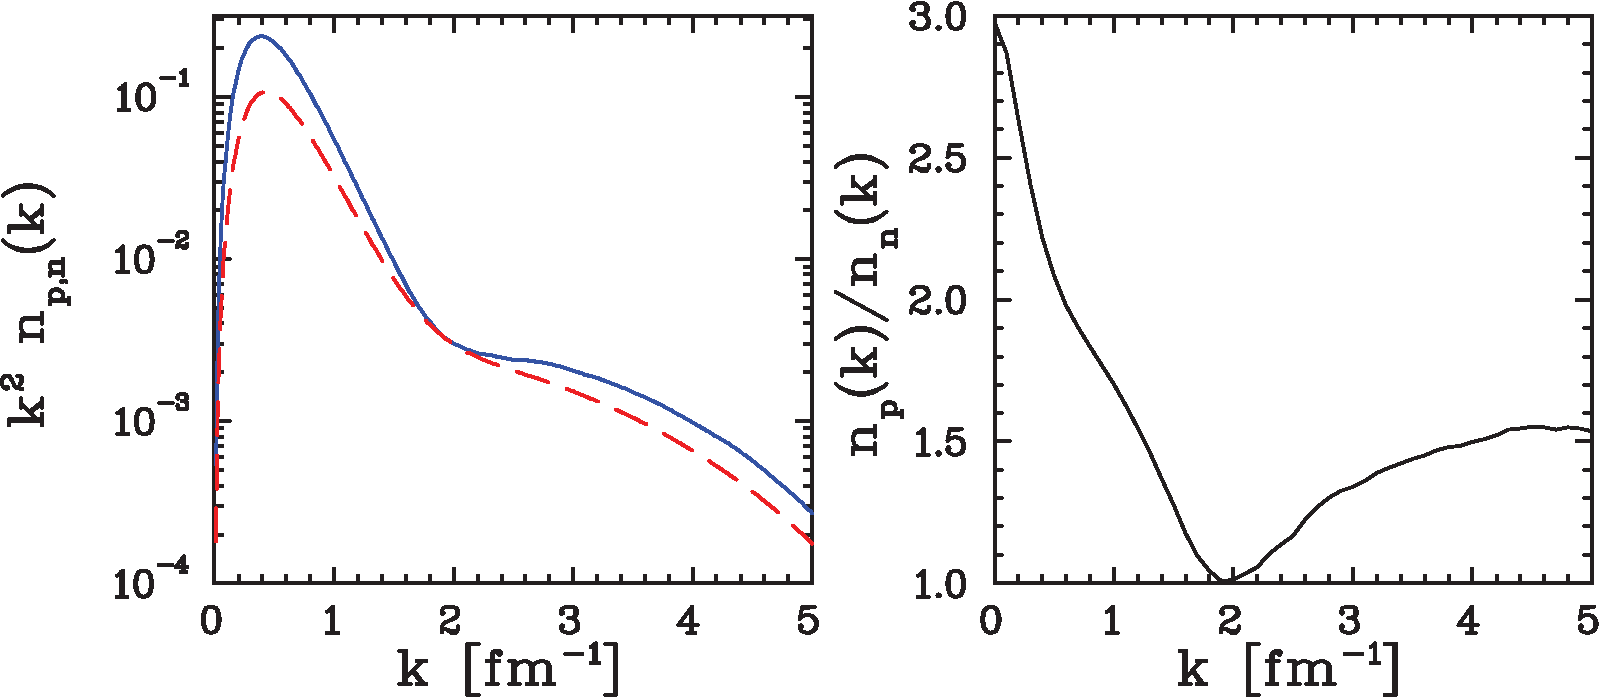
\includegraphics[type=pdf,ext=.pdf,read=.pdf,width=0.90\linewidth]{./figures/physics/mom_dis_np_new}
    \caption[Momentum distribution for proton and neutron and their ratio]{\footnotesize{Left: Momentum distribution for proton (solid) and neutron (dashed) in $\mathrm{^{3}He}$; Right: Ratio of proton to neutron momentum distribution. Plots were originally from Ref.~\cite{Pieper_Wiringa}.}}
    \label{mom_dis_np}
  \end{center}
\end{figure}  
 
\begin{figure}[!ht]
  \begin{center}
    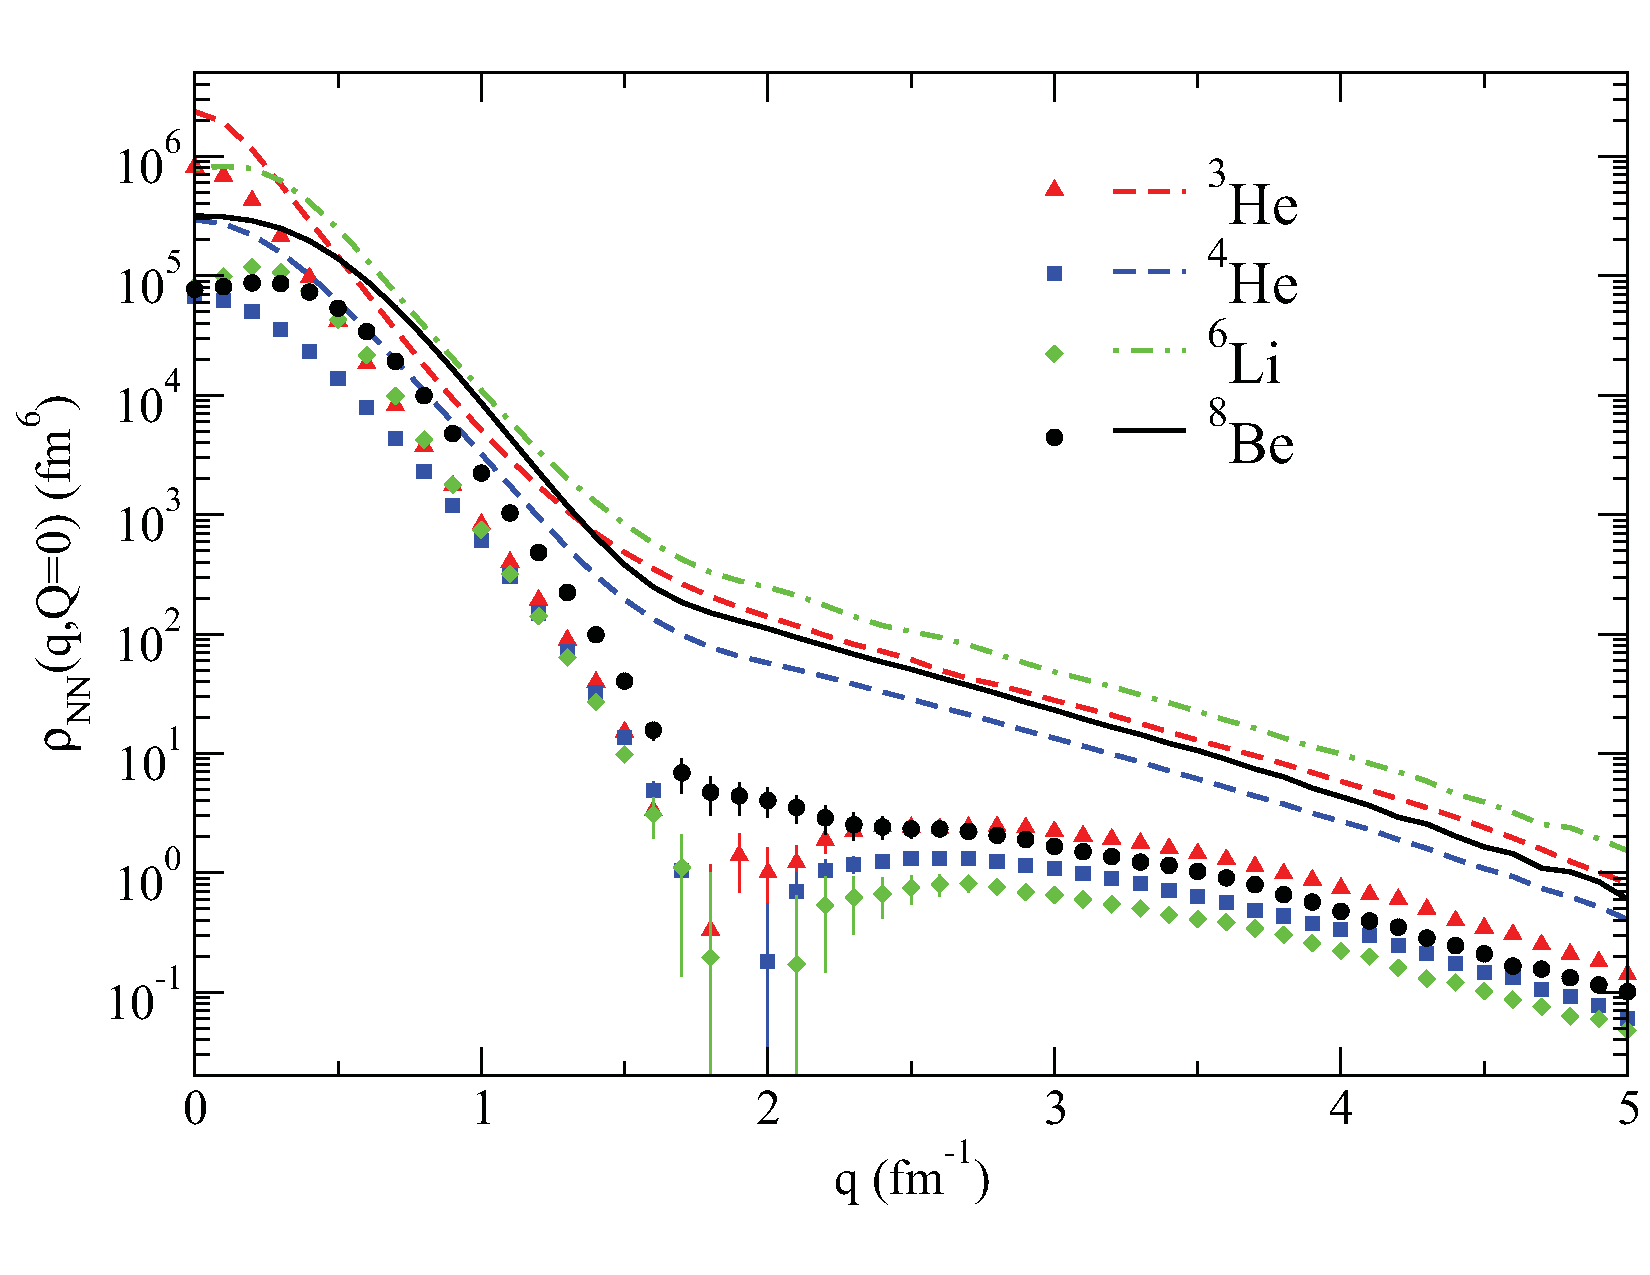
\includegraphics[type=pdf,ext=.pdf,read=.pdf,width=0.60\linewidth]{./figures/physics/isospin_src}
    \caption[Isospin effect in momentum distribution]{\footnotesize{Isospin effect in momentum distribution, where lines represent the momentum distribution in $np$ and dots represent the momentum distribution in $pp$. The unit of the momentum is $\mathrm{fm^{-1}}$ ($\mathrm{1~fm^{-1}\simeq 0.1973~GeV/c}$). Figure is adopted from Ref.~\cite{PhysRevLett.98.132501}.}}
    \label{isospin_src}
  \end{center}
\end{figure} 

Fig.~\ref{mom_dis_np} presents a calculation of the momentum distribution for protons and neutrons and their ratio in $\mathrm{^{3}He}$~\cite{Pieper_Wiringa}. In the assumption of isospin-independence, the momentum ratio of protons to neutrons should be equal to two, but if the SRC is isospin-dependent, the ratio becomes one when the SRC dominates at $k>k_{F}$. The right plot in Fig.~\ref{mom_dis_np} gives a ratio at $k>k_{F}$ roughly equal to 1.5, which suggests that the isospin effect plays a large role in the SRC.

 The reason why $np_{T=0}$ configuration does not totally dominate is that the $T=1$ channels are not completely suppressed, especially at very large momentum, where the 3N-SRC configuration is more complicated. Another calculation extended the study to other nuclei provides similar results~\cite{PhysRevLett.98.132501}. As shown in Fig.~\ref{isospin_src}, the momentum distribution of $np$ pairs is much larger than the one of $pp$ pairs at $300<k<600$ $MeV/c$.

 Inclusive cross sections are also sensitive to the role of isospin. One can examine the isospin-dependence by measuring the cross section ratio of two isotopes at different $\mathrm{Q^{2}}$ in the SRC region. For example, assuming the SRC is independent of the isospin, the cross section of protons to neutrons at large momenta is proportional to N/Z. Considering that the cross section of scattering off a proton is approximately three times larger than the cross section of scattering off a neutron (i.e. $\sigma_{p}\simeq 3\sigma_{n}$), the per nucleon cross section ratio of $\mathrm{^{48}Ca}$ to $\mathrm{^{40}Ca}$ can be written as~\cite{e08014_pr}:
 \begin{equation}
  \frac{\sigma_{^{48}Ca}/48}{\sigma_{^{40}Ca}/40}=\frac{\left(20\sigma_{p}+28\sigma_{n}\right)/48}{\left(20\sigma_{p}+20\sigma_{n}\right)/40}\simeq\frac{\left(20\sigma_{p}+28\sigma_{p}/3\right)/48}{\left(20\sigma_{p}+20\sigma_{p}/3\right)/40}=0.916.
  \label{eq_ca_ratio1}
 \end{equation}

 On the contrary, if the $np$ pairs dominate in the SRC region, one only can compare the cross sections for scattering off nucleons in the $np$ correlations. For $\mathrm{^{40}Ca}$, the maximum number of $np$ pairs is $\mathrm{20\times 20}$, while the number becomes $\mathrm{20\times 28}$ for $\mathrm{^{48}Ca}$. The ratio in Eq.~\eqref{eq_ca_ratio1} becomes:
 \begin{equation}
  \frac{\sigma_{^{48}Ca}/48}{\sigma_{^{40}Ca}/40}=\frac{\left(20\times 28\right)/48}{\left(20\times 20\right)/40}=1.17,
  \label{eq_ca_ratio2}
 \end{equation} 
which is 28\% larger than the ratio with the assumption of isospin independence. 

 However, Eq.~\eqref{eq_ca_ratio2} is a naive calculation since it does not consider the fact that nucleons can only form SRC pairs with their neighbors on account of their short distance properties of NN interactions. The calculations in Ref.~\cite{PhysRevC.84.031302} and \cite{PhysRevC.86.044619} take into account the size effect of $\mathrm{^{48}Ca}$ and $\mathrm{^{40}Ca}$, and predict the ratio in Eq.~\eqref{eq_ca_ratio2} to be near 1.0.
  
  These two Calcium isotopes were used in the E08-014 and the preliminary result will be presented in this thesis. A new proposal~\cite{E12_11_112_pr} in Hall-A at JLab will continue to study the isospin dependence of the SRC with $\mathrm{^{3}He}$ and $\mathrm{^{3}H}$ which have much smaller mass and size differences. The new measurement will provide 40\% deviation of the ratios between the two assumptions about isospin dominance in the SRC. Besides, the ground state wave-functions of $\mathrm{^{3}He}$ and $\mathrm{^{3}H}$ can be calculated exactly, therefore the experimental results will be directly compared with the theoretical models. 

\input ./intro/emc.tex

\section{Final State Interaction in SRC}
A nucleus is a complicated system and the struck nucleon experiences multiple interactions both in its initial and final states. The major problems in the experimental study of the SRC are the FSI, where the momentum and energy of the struck nucleon can be modified during the re-scattering processes with other spectators in the residual system. It is crucial to disentangle the role of the FSI from the SRC in the measurements of electron-nucleon scattering in the nuclei.

 In inclusive electron scattering, the effect from the FSI falls off rapidly at high $\mathrm{Q^{2}}$ as $\mathrm{1/Q^{2}}$~\cite{day_arns,SLAC_Measurement_PRC.48.2451}. At low $\mathrm{Q^{2}}$, the contribution of the FSI is large enough to break down the y-scaling feature of QE scattering in the PWIA~\cite{Day:1987az}. The study of the SRC with inclusive cross section measurements requires sufficiently large $\mathrm{Q^{2}}$ to diminish the FSI contribution. The current results from inclusive data (i.e. in Fig.~\ref{SLAC_2NSRC_xbj}) indicate little dependence of $\mathrm{Q^{2}}$ for the scaling region of the 2N-SRC, which implies that the FSI becomes less important in the kinematic settings of the SRC study ($\mathrm{Q^{2}>1~GeV^{2}}$).

  However, the contribution of the FSI may not completely vanish even at very large $\mathrm{Q^{2}}$. When the electron scatters off a nucleon in a SRC configuration, the struck nucleon may be very close to other correlated nucleons and the probability of re-scattering from the residual system is non-zero. Despite the possible large contributions, they can be removed by taking the cross section ratio if the FSI is localized in the SRC. For example, the FSI contribution in the 2N-SRC pairs in heavy nuclei should be similar to one in $\mathrm{^{2}H}$, and the ratio, $\sigma_{A}/\sigma_{^{2}H}$, should be able to cancel the FSI effect and only yield the clean contribution from the 2N-SRC. 

 Overall, despite that the FSI always exists in the SRC configurations, the effects in a heavy nucleus should be identical to the ones in a light nucleus due to the short distance feature of the SRC configurations. These effects are minimized in the study of the 2N- and 3N-SRC when taking the cross section ratio of heavy nuclei to light nuclei.
%\section{SRC and EMC Effect} 

\section{E08-014 Experiment}
 A new experiment, E08-014~\cite{e08014_pr}, was carried out in 2011 in Hall-A at Jefferson Lab, with an electron beam energy of 3.356 GeV from the continuous electron beam accelerator facility (CEBAF). Utilizing the high resolution spectrometers in their standard configurations, this experiment measured the inclusive cross section of $\mathrm{^{2}H}$, $\mathrm{^{3}He}$, $\mathrm{^{4}He}$, $\mathrm{^{12}C}$, $\mathrm{^{40}Ca}$ and $\mathrm{^{48}Ca}$ at $\mathrm{1.1<Q^{2}<2.5 (GeV/c)^{2}}$, which covered the range of $x_{bj}$ from the QE peak region to above 3.0, as shown in Fig.~\ref{kin_cor}. The absolute cross section results will be used to study the scaling functions and momentum distributions at larger missing momentum, as well as the effect from the FSI. By taking the cross section ratio of heavy targets to $\mathrm{^{2}H}$ or $\mathrm{^{3}He}$, one can examine the $x_{bj}$ and $\mathrm{Q^{2}}$ dependence of the SRC, and measure the values of $a_{2}$ and $a_{3}$. The relatively low $\mathrm{Q^{2}}$ setting allows the study of $\alpha_{2N}$ and $\alpha_{3N}$ in the scaling of SRC. The Calcium isotopes, $\mathrm{^{40}Ca}$ and $\mathrm{^{48}Ca}$, were also used to study the isospin dependence of the 2N- and 3N-SRC. The experimental setup and the data analysis will be described in great details in this thesis and preliminary results will be presented. 
\begin{figure}[!ht]
  \begin{center}
    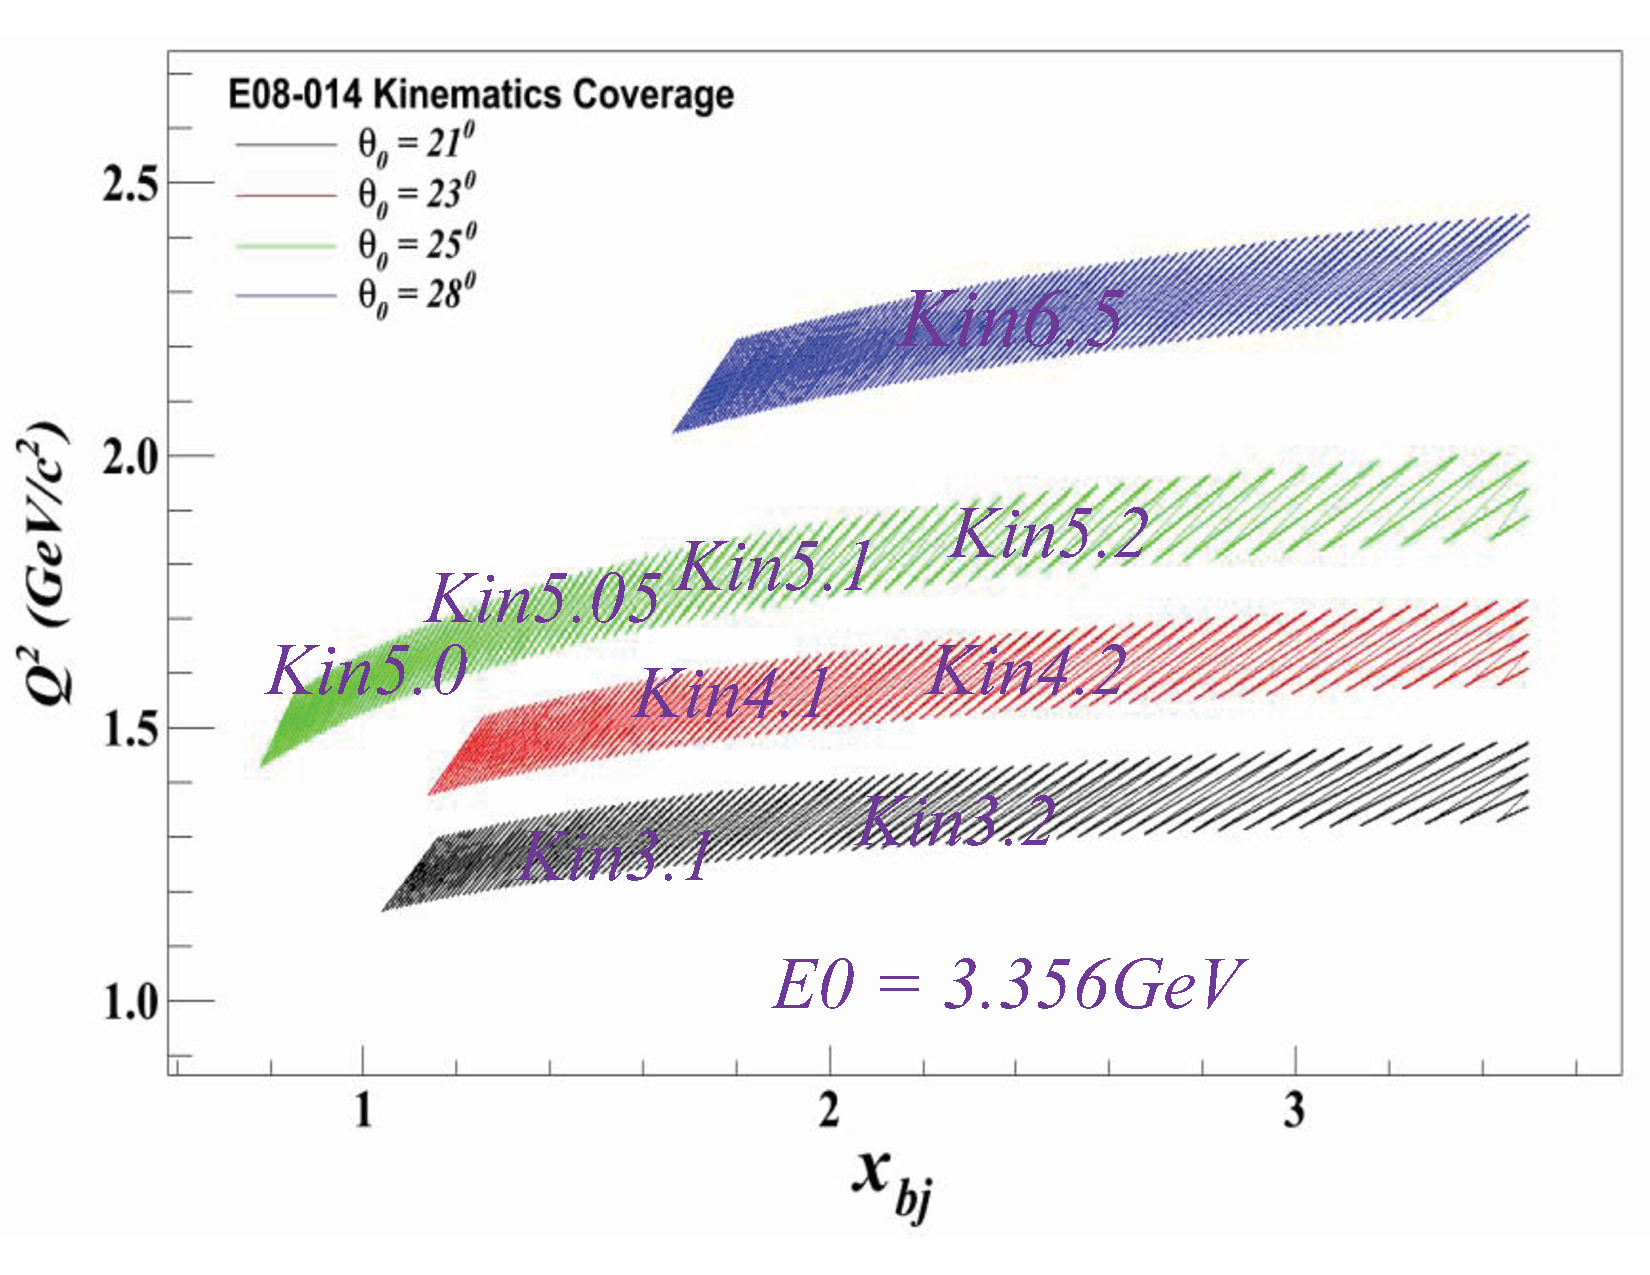
\includegraphics[type=pdf,ext=.pdf,read=.pdf,width=0.70\linewidth]{./figures/physics/E08014_Kin_Cover}
    \caption[Kinematic coverage of the E08-014]{\footnotesize{Kinematic coverage of the E08-014.}}
    \label{kin_cor}
  \end{center}
\end{figure}

